\documentclass[ebook,9pt]{memoir}
\title{pgo}
\author{nick black}
%\special{pdf:minorversion 7}
\usepackage{unicode-math}
\defaultfontfeatures{Scale=MatchUppercase,Ligatures=TeX,Renderer=HarfBuzz}
\usepackage{microtype}
\usepackage{bookmark}
\usepackage{ninecolors}
\usepackage[svgnames,HSB]{xcolor}
\selectcolormodel{rgb}
\usepackage{caption} % for \captionsetup
\usepackage{polyglossia}
\usepackage{pdfpages}
\usepackage{tabularray}
\usepackage{ifthen}
\usepackage{multicol}
\usepackage[siunitx]{circuitikz}
\usepackage[mode=text]{siunitx}
%\usepackage[most]{tcolorbox}
%\usepackage[symbols,notext]{kpfonts-otf} % upsets tex4ebook
\setsansfont{Kanit}
\setmonofont[Scale=0.8]{Hack}
\setmainfont{Gentium Book Plus}
\setdefaultlanguage{american}
\usepackage{newunicodechar}
\usepackage{realscripts} % typographical enhancement for sub/superscripts
\usepackage{luatex85} % otherwise pdfx blows up =\
\usepackage[a-3u]{pdfx}

\settrims{0pt}{0pt}
\setstocksize{8.75in}{5.625in}
\settrimmedsize{8.5in}{5.5in}{*}
\setlrmarginsandblock{.75in}{*}{1}
\setulmarginsandblock{1in}{1in}{1}       % 2" of total vertical margin
\graphicspath{out/}
\setlength{\headwidth}{\textwidth}       % don't go to the end of paperback
\settypeblocksize{6.5in}{\textwidth}{*}   % want 6.5in of our 9/8.5
\checkandfixthelayout                     % print and check layout % W: Command terminated with space. (1)

\newcommand\Midrule[0]{\midrule}

\def\LOGO {\textsf{\fontsize{40pt}{44pt}
  \textbf{
  \begin{center} Quantitative\\
  Pokémon GO
  \end{center}
}}}

\frontmatter
\begin{document}
  \pagestyle{empty}
  \LOGO
  \vfill
  \hrule
  \begin{center}
  \textsf{Gold \& Appel Publishing}
  \end{center}
  \hrule
  \clearpage
  %\input{aux/copyright}
  %\clearpage
  \setcounter{page}{1}
  \pagestyle{plain} % want (roman) page numbers

\ifdefined\epub
\else
  \hypertarget{toc}{}%
  \bookmark[dest=toc]{contents}
  \tableofcontents*
  %\cleartorecto
  \hypertarget{lof}{}%
  \bookmark[dest=lof]{illustrations} % if we use 3, it changes to i instead of iii [shrug]
  \vfill
  \listoftables*
  \listoffigures*
  \fi
%--------------------------main text------------------------------------------%
\mainmatter
\chapter{Foreward}

\noindent{}This text is specific to Pokémon GO, though many details
apply to other games in the Pokémon family.
In particular, it is based on my experimentation with and analysis of
 the 0.361.0 Android release, using decompilation, debuggers, and
 network traffic analysis.
Where possible, I have relied on official Niantic communications
 and my own research.
I attempt to reproduce most claims, though some have been accepted at face value.\\
\\
\noindent{}Changes are frequently made to the game, some of them quite fundamental.
This text documents PGO as it is played in July 2025.
I have not generally bothered to explore variances with historical gameplay.\\
\\
\noindent{}Much of the information herein will be old news to experienced
 PGO players, but I hope that it will provide a valuable reference and central collection of wisdom.
The community established a large body of knowledge long before I
 came to the game.
Still, some of my theories regarding team selection and battle strategy might
  be new to you.
The majority of my novel contributions are found in \autoref{chap:unbounded},
  \autoref{chap:bounded}, and \autoref{chap:simul}.

\chapter{Trainers}
A Pokémon GO account is synonymous with its associated Trainer.

\section{Levels}
\label{sec:levels}
New Trainers start at Level 1 (of 50) with 0 XP\@.
A new Level is conferred as soon as the Trainer's XP meets or exceeds
  that Level's XP threshold (\autoref{table:xp40}).
It is possible to advance multiple Levels via a single award of XP\@.
\begin{table}[hb]
\centering
\begin{tabular}{r r r|r r r}
  Level & kXP & ΔkXP & Level & kXP & ΔkXP \\
\Midrule
1 & 0 & 0 & 21 & 260 & 50 \\
2 & 1 & 1 & 22 & 335 & 75 \\
3 & 3 & 2 & 23 & 435 & 100 \\
4 & 6 & 3 & 24 & 560 & 125 \\
5 & 10 & 4 & 25 & 710 & 150 \\
6 & 15 & 5 & 26 & 900 & 190 \\
7 & 21 & 6 & 27 & 200 & 1,100 \\
8 & 28 & 7 & 28 & 250 & 1,350 \\
9 & 36 & 8 & 29 & 300 & 1,650 \\
10 & 45 & 9 & 30 & 350 & 2,000 \\
11 & 55 & 10 & 31 & 500 & 2,500 \\
12 & 65 & 10 & 32 & 500 & 3,000 \\
13 & 75 & 10 & 33 & 750 & 3,750 \\
14 & 85 & 10 & 34 & 1,000 & 4,750 \\
15 & 100 & 15 & 35 & 1,250 & 6,000 \\
16 & 120 & 20 & 36 & 7,500 & 7,500 \\
17 & 140 & 20 & 37 & 2,000 & 9,500 \\
18 & 160 & 20 & 38 & 2,500 & 12,000 \\
19 & 185 & 25 & 39 & 3,000 & 15,000 \\
20 & 210 & 25 & 40 & 5,000 & 20,000 \\
\end{tabular}
\caption{Requirements for Trainer Levels 1--40}
\label{table:xp40}
\end{table}
Levels 41 and above have extra requirements beyond XP (\autoref{table:xp41plus}).
\begin{table}[ht]
\centering
  \begin{tabular}{rrrp{0.65\textwidth}}
Level & MXP & ΔMXP & Special requirements \\
\Midrule
41 & 26 & 6 & 20 Legendary/Mythical power ups,\newline
                      30 raid wins, 5 Gold medals,\newline
                      200 Pokémon caught in 24 hours\\
42 & 33.5 & 7.5 & Evolve all 8 Eevee forms, 3 excellent throws,\newline
                      200 Pokémon caught with berries,\newline
                      15 item-assisted evolutions\\
43 & 42.5 & 9 & 100 Stardust earned,
                      200 effective Charged Attacks,
                      5 Legendary/Mythical catches,
                      5 Platinum medals \\
44 & 53.5 & 11 & 30 Great League wins,
                       30 Ultra League wins,
                       30 Master League wins,
                       20 GO Battle League battles \\
45 & 66.5 & 13 & 100 GO Rocket Grunt wins,
                       100 Pokémon purified,
                       50 GO Rocket Leader wins,
                       10 Platinum medals\\
46 & 82 & 15.5 & 100 Field Research tasks,
                       7 consecutive days w/snapshot,
                       50 Excellent throws,
                       30 Eggs hatched\\
47 & 100 & 18 & 30 raid wins with heterogenous teams,\newline
                        3🟉+ Raid win with CP1500-bounded team,\newline
                        3 power ups to Max CP, 20 Platinum medals\\
48 & 121 & 21 & 10 Souvenirs from buddy,
                        300 hearts with buddy,
                        200 km walked with buddy,
                        8 weeks with 25 km walked\\
49 & 146 & 25 & 10 trades of 300 km+ catch distance,
                        50 Lucky Pokémon received in trades,
                        500 Gifts sent,
                        35 Platinum medals\\
50 & 176 & 30 & 999 Excellent throws,
                        5 consecutive Legendary/Mythical catches,
                        3 GO Rocket Leader wins with CP2500-bounded teams,
                        Rank 10 in GO Battle League\\
\end{tabular}
\caption{Requirements for Trainer Levels 41--50}
\label{table:xp41plus}
\end{table}
Certain elements of gameplay are gated by Trainer Level (\autoref{table:levelgates}),
  and a Trainer cannot control Pokémon whose Level exceeds the Trainer's
  by more than 10---a Level 22 Trainer will be unable to power up (\autoref{sec:plevel}) a Pokémon past Level 32.
Reaching a new Level is rewarded with items (\autoref{table:levelitems}).
Levels 7, 8, 15, and 20 introduce Special Research (\autoref{sec:research}).
\begin{table}[ht]
  \centering
  \begin{tabular}{r p{0.75\textwidth}}
  Level & Features unlocked \\
\Midrule
  2 & Nenab berries \\
  5 & Potions, Revives, Teams, Appraisal, Gyms, Raids \\
  8 & Razz berries, Team GO Rocket \\
  10 & Super Potions, Golden Razz berries, Evolution items, Trades, Trainer Battles \\
  12 & Great Balls \\
  15 & Hyper Potions, Fast TMs, Parties \\
  18 & Pinap berries \\
  20 & Silver Pinap berries, Ultra Balls, Mega Evolution \\
  25 & Max Potions, Charged TMs \\
  30 & Max Revives, Route submission \\
  31 & XL Candy \\
  37 & Pokéstop submission \\
\end{tabular}
\caption{Features unlocked by Trainer Levels}
\label{table:levelgates}
\end{table}
\begin{table}[h!]
\centering
\setlength{\tabcolsep}{1pt}
\footnotesize
\begin{tabular}{r|g c g c g c g c g c g c g c g c g c g c g c g}
&

\includegraphics[width=1em]{images/pokeball.png} &

\includegraphics[width=1em]{images/greatball.png} &

\includegraphics[width=1em]{images/ultraball.png} &

\includegraphics[width=1em]{images/nanab.png} &

\includegraphics[width=1em]{images/razz.png} &

\includegraphics[width=1em]{images/pinap.png} &

\includegraphics[width=1em]{images/silverpinap.png} &

\includegraphics[width=1em]{images/incense.png} &

\includegraphics[width=1em]{images/revive.png} &

\includegraphics[width=1em]{images/maxrevive.png} &
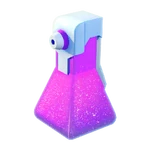
\includegraphics[width=1em]{images/Potion.png} &

\includegraphics[width=1em]{images/superpotion.png} &
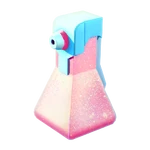
\includegraphics[width=1em]{images/Hyper_Potion.png} &

\includegraphics[width=1em]{images/Max_Potion.png} &
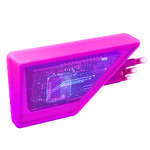
\includegraphics[width=1em]{images/lure.png} &

\includegraphics[width=1em]{images/luckyegg.png} &

\includegraphics[width=1em]{images/rarecandy.png} &
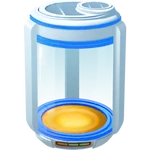
\includegraphics[width=1em]{images/incubatorlimited.png} &
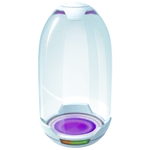
\includegraphics[width=1em]{images/incubatorsuper.png} &

\includegraphics[width=1em]{images/rarecandyxl.png} &

\includegraphics[width=1em]{images/pokecoin.png} &
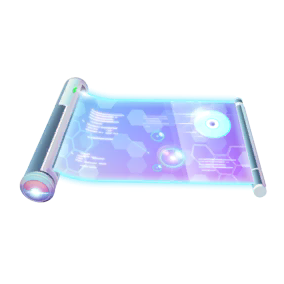
\includegraphics[width=1em]{images/elitefasttm.png} &
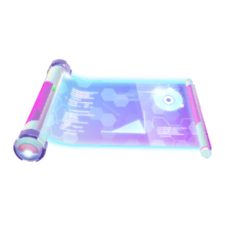
\includegraphics[width=1em]{images/elitechargedtm.png}
  \\
  2 & 10 &    &    &  6 &    &    &    &   &    &    &    &    &    &    &   &   &    &   &   &   &   &   &   \\
  3 & 15 &    &    &  8 &    &    &    &   &    &    &    &    &    &    &   &   &    &   &   &   &   &   &   \\
  4 & 15 &    &    & 15 &    &    &    &   &    &    &    &    &    &    &   &   &    &   &   &   &   &   &   \\
  5 & 20 &    &    &    &    &    &    & 1 & 10 &    & 10 &    &    &    &   &   &    &   &   &   &   &   &   \\
  6 & 15 &    &    &    &    &    &    &   &  5 &    & 10 &    &    &    &   &   &    & 1 &   &   &   &   &   \\
  7 & 15 &    &    &    &    &    &    & 1 &  5 &    & 10 &    &    &    &   &   &    &   &   &   &150&   &   \\
  8 & 15 &    &    &    & 10 &    &    &   &  5 &    & 10 &    &    &    & 1 &   &    &   &   &   &   &   &   \\
  9 & 15 &    &    &    &  3 &    &    &   &  5 &    & 10 &    &    &    &   & 1 &    &   &   &   &   &   &   \\
  10 & 20 &    &    &    & 10 &    &    & 1 & 10 &    &    & 20 &    &    & 1 & 1 &    & 1 &   &   &   &   &   \\
  11 & 15 &    &    &    &  3 &    &    &   &  3 &    &    & 10 &    &    &   &   &    &   &   &   &   &   &   \\
  12 &    & 20 &    &    &  3 &    &    &   &  3 &    &    & 10 &    &    &   &   &    &   &   &   &   &   &   \\
  13 &    & 10 &    &    &  3 &    &    &   &  3 &    &    & 10 &    &    &   &   &    &   &   &   &   &   &   \\
  14 &    & 10 &    &  3 &    &    &    &   &  3 &    &    & 10 &    &    &   &   &    &   &   &   &   &   &   \\
  15 &    & 15 &    &    & 10 &    &    & 1 & 10 &    &    &    & 20 &    & 1 & 1 &    & 1 &   &   &   &   &   \\
  16 &    & 10 &    &  5 &    &    &    &   &  5 &    &    &    & 10 &    &   &   &    &   &   &   &   &   &   \\
  17 &    & 10 &    &    &  5 &    &    &   &  5 &    &    &    & 10 &    &   &   &    &   &   &   &   &   &   \\
  18 &    & 10 &    &    &    &  5 &    &   &  5 &    &    &    & 10 &    &   &   &    &   &   &   &   &   &   \\
  19 &    & 15 &    &    &  5 &    &    &   &  5 &    &    &    & 10 &    &   &   &    &   &   &   &   &   &   \\
  20 &    &    & 20 & 20 &    &    &    & 2 & 20 &    &    &    & 20 &    & 2 & 2 &    & 2 &   &   &   &   &   \\
  21 &    &    & 10 &    &    & 10 &    &   & 10 &    &    &    & 10 &    &   &   &    &   &   &   &   &   &   \\
  22 &    &    & 10 &    & 10 &    &    &   & 10 &    &    &    & 10 &    &   &   &    &   &   &   &   &   &   \\
  23 &    &    & 10 & 10 &    &    &    &   & 10 &    &    &    & 10 &    &   &   &    &   &   &   &   &   &   \\
  24 &    &    & 15 &    & 10 &    &    &   & 10 &    &    &    & 10 &    &   &   &    &   &   &   &   &   &   \\
  25 &    &    & 25 &    &    & 15 &    & 1 & 15 &    &    &    &    & 20 & 1 & 1 &    & 1 &   &   &   &   &   \\
  26 &    &    & 10 &    & 15 &    &    &   & 10 &    &    &    &    & 15 &   &   &    &   &   &   &   &   &   \\
  27 &    &    & 10 & 15 &    &    &    &   & 10 &    &    &    &    & 15 &   &   &    &   &   &   &   &   &   \\
  28 &    &    & 10 &    & 15 &    &    &   & 10 &    &    &    &    & 15 &   &   &    &   &   &   &   &   &   \\
  29 &    &    & 10 &    &    & 15 &    &   & 10 &    &    &    &    & 15 &   &   &    &   &   &   &   &   &   \\
  30 &    &    & 30 &    & 20 &    &    & 3 &    & 20 &    &    &    & 20 & 3 & 3 &    & 3 &   &   &   &   &   \\
  31 &    &    & 10 & 15 &    &    &    &   &    & 10 &    &    &    & 15 &   &   &    &   &   &   &   &   &   \\
  32 &    &    & 10 &    & 15 &    &    &   &    & 10 &    &    &    & 15 &   &   &    &   &   &   &   &   &   \\
  33 &    &    & 10 &    &    & 15 &    &   &    & 10 &    &    &    & 15 &   &   &    &   &   &   &   &   &   \\
  34 &    &    & 10 &    & 15 &    &    &   &    & 10 &    &    &    & 15 &   &   &    &   &   &   &   &   &   \\
  35 &    &    & 30 & 20 &    &    &    & 2 &    & 20 &    &    &    & 20 & 1 & 1 &    & 1 &   &   &   &   &   \\
  36 &    &    & 20 &    & 20 &    &    &   &    & 10 &    &    &    & 20 &   &   &    &   &   &   &   &   &   \\
  37 &    &    & 20 &    &    & 20 &    &   &    & 10 &    &    &    & 20 &   &   &    &   &   &   &   &   &   \\
  38 &    &    & 20 &    & 20 &    &    &   &    & 10 &    &    &    & 20 &   &   &    &   &   &   &   &   &   \\
  39 &    &    & 20 & 20 &    &    &    &   &    & 10 &    &    &    & 20 &   &   &    &   &   &   &   &   &   \\
  40 &    &    & 40 &    & 40 &    &    & 4 &    & 40 &    &    &    & 40 & 4 & 4 &    & 4 &   &   &   &   &   \\
  41 &    &    & 20 &    & 20 &    &    &   &    & 20 &    &    &    & 20 &   &   & 1  & 1 &   & 1 &   &   &   \\
  42 &    &    & 20 & 20 &    &    &    &   &    & 20 &    &    &    & 20 &   &   & 1  & 1 &   & 1 &   &   &   \\
  43 &    &    & 20 &    &    &    & 20 &   &    & 20 &    &    &    & 20 &   &   & 1  & 1 &   & 1 &   &   &   \\
  44 &    &    & 20 &    & 20 &    &    &   &    & 20 &    &    &    & 20 &   &   & 1  & 1 &   & 1 &   &   &   \\
  45 &    &    & 40 &    &    &    &    & 2 &    & 40 &    &    &    &    & 2 & 2 & 1  &   & 1 & 2 &   & 1 &   \\
  46 &    &    & 30 &    & 25 &    &    &   &    & 20 &    &    &    & 25 &   &   & 1  & 1 &   & 1 &   &   &   \\
  47 &    &    & 30 & 25 &    &    &    &   &    & 20 &    &    &    & 25 &   &   & 1  & 1 &   & 1 &   &   &   \\
  48 &    &    & 30 &    &    &    & 15 &   &    & 20 &    &    &    & 25 &   &   & 1  & 1 &   & 1 &   &   &   \\
  49 &    &    & 30 &    &    & 25 &    &   &    & 20 &    &    &    & 25 &   &   & 1  & 1 &   & 1 &   &   &   \\
  50 &    &    & 50 &    &    &    &    & 5 &    &    &    &    &    & 50 & 5 & 5 & 2  &   & 5 & 2 &   &   & 1 \\
\end{tabular}
\caption{Items awarded for reaching Trainer Levels}
\label{table:levelitems}
\end{table}
All level-gated mechanics, including the ability to fully power up Pokémon,
 are available at Level 40\footnote{The maximum Pokémon Level is 50 (\autoref{chap:pokemon}).}.
Levels 43, 45, 48, and 50 provide extra Challenge quests.
Levels 41, 43, 45, 47, 49, and 50 open some cosmetic options for Trainer avatars.
Trainer Level determines the maximum level of wild spawns
  (\autoref{sec:spawns}) and the difficulty of Team GO Rocket
  opponents (\autoref{sec:rocket}).

\section{Team}
Upon reaching Level 5, a Trainer can join one of three Teams: Mystic (blue),
  Valor (red), or Instinct (yellow).
The only non-cosmetic effect of Team choice regards Gyms (\autoref{sec:gyms}), which
  are held by one Team at a time.
A Trainer can change their Team by purchasing and making use of a Team Medallion.
The cost is 1,000 Pokécoins, and 365 days must pass between Medallion purchases.

It seems sadly impossible to join GO Rocket. Alas!

\section{Capacities}
\label{sec:capacities}
A Trainer enters this world with no Pokémon, no Pokécoins, no Stardust,
  no Max Particles, no Candy of any kind, no Mega Energy of any kind,
  no Primal Energy of any kind, no Fusion Energy of any kind, and no Crown
  Energy of any kind.
They have initial carrying capacity sufficient for 300 Pokémon.
Additional storage can be added in increments of 50, up to a total of 10,500.
Each upgrade costs 200 Pokécoins.
A full upgrade will thus currently run you 40,800 Pokécoins.

The Trainer has a Bag capable of storing 350 items (strangely, not all items
  count against this limit, including Gifts, Stickers, and the Postcard Book,
  which I suppose are shoved down the front of one's Trainer uniform).
The Bag comes with an Infinite Incubator, a Camera, 2 Incense, and 50 Poké Balls,
  and thus space for 296 new items.
The Bag can be upgraded to store up to 9,500 items.
Here again, each upgrade costs 200 Pokécoins, and increases capacity by 50 items.
The maximum Bag is thus 36,600 Pokécoins.

The Trainer has a Postcard Book with seven pages, each capable of retaining
 50 Postcards, for an inital limit of 350.
Pages can be added for 100 Pokécoins each, up to a maximum of 40 Pages
 supporting 2,000 total Postcards.
Such a monster will cost 3,300 Pokécoins.

The Trainer can carry up to twenty Gifts at a time. and up to 25 of each sticker.
To date, no one has found any use for the stickers.

Upon obtaining four Shadow Shards, they are automatically refined into a Purified Gem.
The Trainer can carry up to ten Purified Gems.
Shadow Shards cannot be collected while holding ten gems, though any extras
 following the tenth gem's purification will be retained (this can only
 happen when receiving multiple shards in a single award).

The Trainer can accumulate no more than 9,999 units of a given Mega Energy,
 Primal Energy, or Fusion Energy.
A limit on Crown Energy is not yet known, but seems likely to be 9,999.

No limit is known for Candy nor Candy XL.
A lower bound has been established in the millions.
It seems plausible that the limit is one less than a large power of 2:
  2,147,483,647 seems as good a guess as any\footnote{If the limit is driven by UI requirements, it's likely lower.}.

\section{Pokédexen}
\label{sec:dexen}
The Trainer has ten Pokédexen\footnote{``Pokédexes'' to the uncultured.}:
  ``Pokémon'', ``Shiny'', ``XXL'', ``XXS'', ``G-Max'', ``Mega'', ``Shadow'',
  ``Purified'', ``🟉100\%'', and ``Lucky''.
All ten start empty, and several start locked.
\textbf{FIXME details}
Entries are filled in as the relevant Pokémon are acquired (via any means).
Once registered, Pokédex entries are never unregistered.
If an entry is made in some Pokédex, the corresponding entry is also made
  in the primary Pokédex.
Shiny Shadow Pokémon and Shiny Purified Pokémon are registered to the
  ``Shiny'' Pokédex along with the ``Shadow'' or ``Purified'' Pokédex.

Besides pointless nostalgia, the ``Info'' and ``Battle'' tabs of filled entries
  provide information regarding evolution (\autoref{sec:evolution}), type
  relations (\autoref{chap:types}), and attacks (\autoref{chap:attacks}).
Trainers can place an alert on one filled or silhouetted entry to receive
  notifications when that Pokémon is nearby.
Some extreme collectors maintain ``living Pokédexen'', i.e. one of each
  species/form (sometimes with extra requirements) in their usable Pokémon storage.

\section{Grinding}
\label{sec:grinding}
For me, the joy of Pokémon GO is almost entirely found in its PvP League play (\autoref{sec:3x3}).
Others take pleasure from its collection and social aspects.
Either way, you'll be doing a good bit of slogging in order to find, develop,
  and evolve powerful Pokémon.
Those willing to spend money can speed the process up a bit, but there's
  no escaping the fundamental cycles of Catch, Appraise, Transfer and
  Catch, Appraise, Develop. 
I began playing on 2025-03-01.
As I write this about four months later, I have caught 20,364 Pokémon, of which
  I have retained 441---a little less than 2.2\%.

\subsection{Collecting Pokémon}
\label{subsec:getmons}
Pokémon can be received from other Trainers via trades (\autoref{sec:trades}),
  but most are captured with Pokéballs in encounters.
An encounter involves a single subject Pokémon, a single Trainer,
  and possibly that Trainer's current Buddy Pokémon.
Outcomes (aside from certain plot-based encounters) include capture, flight of
  the Pokémon, and departure of the Trainer.

During the initial tour with Professor Willow, you select one of
 Bulbasaur, Charmander, Squirtle, or Pikachu to catch.
You will enter the Encounter screen, be provided an infinite supply of
  Pokéballs for the encounter, and enjoy a catch rate (\autoref{sec:catch}) set to 100\%.

Pokémon will spawn on the Map screen, seemingly at random (see \autoref{sec:spawns} for details).
Pressing on them will open the Encounter screen with that Pokémon,
  providing an opportunity to catch it.
Encounters are also triggered by the completion of certain Research,
  defeats of Team GO Rocket, Raid wins, and Max Battle wins.
Encounters due to Research can be arbitrarily postponed by leaving the encounter screen,
  or simply not closing the research out.
Leaving wild encounters might see the Pokémon disappear from the Map, especially
  if you've moved significantly, or much time has gone by.
Encounters following battle wins are one-and-done; if you exit the encounter,
  that Pokémon is gone.

\subsection{Collecting XP}
\label{subsec:getxp}
Gaining sufficient XP advances the Trainer's level.
It is most regularly received for capturing Pokémon, but large awards are
  available by other means, and can be the source of a majority of a Trainer's XP.
  \textbf{FIXME}
Using a Lucky Egg doubles all XP awards for thirty minutes.
During this time, a timer appears on the upper right of the map screen.
Lucky Eggs can be bought from the Shop (one for 80 Pokécoins or eight for 500),
  and are sometimes awarded for completing Research.

%\begin{figure}[h]
%  \begin{minipage}[t]{0.3\textwidth}
%    \begin{center}
%    
\includegraphics[width=\textwidth]{images/luckyegg.png}
%    \end{center}
%    \caption*{Lucky egg}
%    \label{fig:luckyegg}
%  \end{minipage}
%  \begin{minipage}[t]{0.3\textwidth}
%    \begin{center}
%    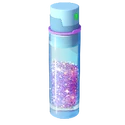
\includegraphics[width=\textwidth]{images/stardust.png}
%    \end{center}
%    \caption*{Stardust}
%    \label{fig:stardust}
%  \end{minipage}
%  \begin{minipage}[t]{0.3\textwidth}
%    \begin{center}
%    
\includegraphics[width=\textwidth]{images/starpiece.png}
%    \end{center}
%    \caption*{Star piece}
%    \label{fig:starpiece}
%  \end{minipage}
%\end{figure}
%
\subsection{Collecting Stardust}
\label{subsec:getdust}
Trainers pay a cost (partially) in Stardust
  to level up their Pokémon (\autoref{sec:plevel}),
  to trade them (\autoref{sec:trades}),
  to purify Shadow Pokémon (\autoref{sec:shadow}),
  to teach them second charged attacks (\autoref{sec:charged}),
  to change certain forms (\autoref{sec:forms}),
  and to activate Adventure Effects (\autoref{sec:effects}).
Stardust becomes the primary bottleneck on advancement fairly early in the game:
  Pokémon at higher levels require more Stardust to power up (\autoref{table:powerups}),
  but the amount of Stardust awarded for their capture doesn't change.
There is never enough, and one must carefully manage its use.

The primary means of acquiring Stardust is catching Pokémon.
The vast majority of Pokémon result in one of three awards based on their stage
 (\autoref{sec:evolution}), but a few offer more (\autoref{table:stardust}),
 making them excellent targets for Razz berries.
A Pokémon which is weather-boosted (\autoref{sec:weather}) awards 25\% more than normal.
Stardust can also be collected for wins in the GO Battle League,
  opening Gifts (\autoref{sec:gifts}),
  completing Routes,
  completing Research,
  participating in Showcases,
  defeating Team Leaders in Trainer Battles,
  defeating Team GO Rocket,
  hatching eggs,
  feeding berries to Pokémon defending your team's Gyms (30 per),
  and from weekly Adventure Sync rewards based on the total distance walked.
5🟉 and 6🟉 Max Battles award 15,000 and 25,000 Stardust respectively.
\begin{table}[ht]
\centering
\begin{tabular}{p{.75\textwidth}rr}
Pokémon & Award & w/boost\\
\Midrule
Audino & 2100 & 2625\\
Cloyster & 1200 & 1500\\
Shellder, Chimecho & 1000 & 1250\\
Alolan Persian, Starmie, Vespiquen, Garbodor & 950 & 1188\\
Alolan Meowth, Staryu, Sableye, Combee, Trubbish & 750 & 938\\
Parasect, Persian, Breloom, Amoonguss, Shiinotic & 700 & 875\\
Paras, Meowth, Delibird, Shroomish, Foongus,\newline
\hspace{\parindent}Morelull, and stage 3 Pokémon not yet specified & 500 & 625\\
Stage 2 Pokémon not yet specified & 300 & 375\\
All other Pokémon & 100 & 125\\
\end{tabular}
\caption{Stardust awards for capturing Pokémon}
\label{table:stardust}
\end{table}
Using a Star Piece increases all Stardust awards by 50\% for thirty minutes.
During this time, a timer appears on the upper right of the map screen.
Star Pieces can be bought from the Shop (one for 100 Pokécoins or eight for 640),
  and are sometimes awarded for completing Research.
\subsection{Collecting Candy}
\label{subsec:getcandy}
Each genus (\autoref{sec:evolution}) has its own flavor of Candy and Candy XL.
Along with Stardust, most Pokémon enhancement is driven by Candy.
Candy is primarily acquired by capturing Pokémon: each capture (in any context)
  awards Candy (and possibly Candy XL) of the capture's genus.
Three Candy are awarded for capture of a Stage 1 Pokémon, five for a Stage 2,
  and ten for Stage 3.
Pinap and Silver pinap berries increase this award (\autoref{sec:berries}).
Candy XL is necessary for advancing Pokémon past Level 40.
100 Candy can be exchanged for a single Candy XL of that same flavor.
Each Rare Candy can be converted into arbitrarily flavored Candy; Rare Candy XL can become any flavor of Candy XL\@.

A Pokémon can be ``transferred to the Professor'' for soul harvesting;
  its loss of existence is your gain of one tasty Candy.
Certain plot armored Pokémon cannot be harvested (\autoref{sec:myths}).
If a Pokémon HOME account is linked, Pokémon can likewise be transferred there,
  resulting in a single Candy.
Evolution consumes many Candies, but returns one when complete.

Walking with a Buddy (\autoref{sec:buddies} will generate Candy (and possibly Candy XL).
The distance that must be walked depends on the Buddy's cost group (\autoref{sec:costgroups}).
Giving berries to gym defenders rarely results in Candy (in addition to guaranteed XP and Stardust).
Hatching an egg yields Candy of the hatched genus, depending on the egg type.
It is possible through Research to receive Candy for a genus not present in
  your Pokédex, i.e. one whose constituent species you have never captured.
You'll keep this Candy, but it doesn't result in a Pokédex entry.
Likewise, Candy is retained even if all Pokémon of that genus have been transferred.
\subsection{Collecting Energies}
The relevant Energies (Mega, Primal, Fusion, and Crown) can be acquired by winning a raid of that type,
  walking with a Mega Evolved or Primal Reverted Buddy, and completing
  certain research tasks.
Note that Mega and Primal evolutions are temporary, while Fusion and Crowning is persistent
  until explicitly undone.
\subsection{Collecting Pokécoins (and F2P vs. P2P)}
\label{subsec:getcoins}
Pokémon GO is free to download, with optional microtransactions through the ingame
  Shop and the Pokémon GO web store.
Pokécoins can be used to purchase most items\footnote{Event passes generally require cash,
  as do some web store bundles.}, and local currency can purchase Pokécoins.
Interestingly, the ratio of exchange rates for Pokécoin and USD diverges
  wildly across regions.
It should be noted that use of e.g. a VPN to purchase Pokécoins remotely is a
  violation of the TOS.
A one-time award of 150 Pokécoins---a humble sum---is presented upon reaching Level 7,
  mainly to ensure Trainers are aware of the game's spending opportunities.
More usefully, Pokémon defeated while defending a Gym (\autoref{sec:gyms}) can
  return with Pokécoins.
The Pokémon receives one Pokécoin for every ten minutes spent in the Gym,
  and presents these weregild to the Trainer upon return.
The Trainer can collect only 50 Pokécoin each calendar day, no matter how many Pokémon return.
This maximum is achieved by 8⅓ hours' occupancy of Gyms.

As an example, a Trainer leaves Pokémon in aligned gyms at 2200h and 2210h local time.
The first returns at 2341h that evening, the second at 1001h the next morning.
The Trainer receives 10 Pokécoins at 2341h, and 50 Pokécoins at 1001h, for a total of 60.
If the first returned instead at 0001h, the Trainer would receive 12 Pokécoins at 0001h,
  and 38 Pokécoins at 1001h, for a total of 50.
Note that the second case earns less, despite greater occupancy time.
By regularly taking Gyms, with a little luck a Trainer can accumulate 350 free Pokécoins each week.

Is it possible to play PGO at a high level without spending money?
The serious collector-style Trainer has costs related to storage and raiding (\autoref{sec:raids})
  that can't be easily met by 350 Pokécoins per week, especially
  in pursuit of Shiny Pokémon (\autoref{sec:shiny}),
  but millions of people collect at a hobbyist level for free.
For the PvP-oriented Trainer, there's little need to spend at all,
  especially if you live in an area with lots of PGO activity.
I have minimal Bag and Pokémon storage (800 and 500 respectively), and raid almost exclusively locally using the daily free pass.
Very few of my Pokémon have the optimal IVs for their Leagues (\autoref{chap:bounded}),
  and I don't yet have many of the Pokémon with which I'd like to experiment,
  yet my Great and Ultra League Elos rarely dip below 2300.
Frankly, I consider my free play a point of pride\footnote{I've spent a little less than 80 USD to date.}.
Whether one needs spend money in Pokémon GO is entirely a matter of goals, dedication, and patience.
With that said, if you want to spend, go with God---thanks for making my free play possible.

The calculus changes for rural Trainers.
Without local raiding (and at least four or five other Trainers to join on larger battles),
  it will be difficult to collect a diverse team of competitive Pokémon.
There are two alternatives: trading (\autoref{sec:trades}), which requires meeting Trainers
  already in possession of the desired Pokémon, and remote raiding.
Remote raiding requires passes, which require Pokécoins---525 for 3 passes at this time.
Collecting the maximum 50 from Gyms eleven out of every fourteen days, you can do
  three free remote raids every two weeks.
Only you know whether that can satisfy your needs.

\section{Medals}
\label{sec:medals}
There is a large set of Medals---most of them functionally meaningless---each of which can be achieved at the Bronze,
 Silver, Gold, or Platinum level.
\begingroup
\setlength{\tabcolsep}{1pt}
\footnotesize
\begin{longtable}{m{.3\textwidth}m{.4\textwidth}rrrr}
Name & Counts & B & S & G & P\\
\Midrule
\endhead
Jogger & km walked & 10 & 100 & 1k & 10k\\
Collector & Captures & 30 & 500 & 2k & 50k\\
Scientist & Evolutions & 3 & 20 & 200 & 2k\\
Breeder & Hatches & 10 & 100 & 500 & 2.5k\\
Backpacker & Pokéstop spins & 100 & 1k & 2k & 50k\\
Sightseer & Unique Pokéstops & 10 & 100 & 1k & 2k\\
Fisher & Large Magikarp captures & 3 & 50 & 300 & 1k\\
Battle Girl & Gym battle wins & 10 & 100 & 1k & 4k\\
Ace Trainer & Team Leaders wins & 10 & 100 & 1k & 2k\\
Youngster & Tiny Rattate captures & 3 & 50 & 300 & 1k\\
Pikachu Fan & Pikachu captures & 3 & 50 & 300 & 1k\\
Unown & Unique Unown captures & 3 & 10 & 26 & 28\\
Champion & 4🟉- raid wins & 10 & 100 & 1k & 2k\\
Battle Legend & 5🟉+ raid wins & 10 & 100 & 1k & 2k\\
Berry Master & Gym berry feeds & 10 & 100 & 1k & 15k\\
Gym Leader & Gym occupancy hours & 10 & 100 & 1k & 15k\\
Pokémon Ranger & Field Research & 10 & 100 & 1k & 2.5k\\
Idol & Best Friends & 1 & 2 & 3 & 20\\
Gentleman & Trades & 10 & 100 & 1k & 2.5k\\
Pilot & km of Trades & 1k & 100k & 1M & 10M\\
Great League Veteran & GL wins & 5 & 50 & 200 & 1k\\
Ultra League Veteran & UL wins & 5 & 50 & 200 & 1k\\
Master League\newline{}Veteran & ML wins & 5 & 50 & 200 & 1k\\
Cameraman & Snapshot photobombs & 10 & 50 & 200 & 400\\
Purifier & Purifications & 5 & 50 & 500 & 1k\\
Hero & GO Rocket Grunt\newline{}and Leader wins & 10 & 100 & 1k & 2k\\
Ultra Hero & Giovanni wins & 1 & 5 & 20 & 50\\
Best Buddy & Best Buddies & 1 & 10 & 100 & 200\\
Wayfarer & Wayfarer agreements & 50 & 500 & 1k & 1.5k\\
Triathlete & 7-day streaks & 1 & 10 & 50 & 100\\
Rising Star & Unique raid wins & 2 & 10 & 50 & 150\\
Rising Star Duo & Raid wins w/friends & 10 & 100 & 1k & 2k\\
Picnicker & Pokémon spawned due your Lures, captured by other Trainers & 5 & 25 & 500 & 2.5k\\
Successor & Mega evolutions & 1 & 50 & 500 & 1k\\
Mega Evolution Guru & Unique Mega evolutions & 1 & 24 & 36 & 46\\
Friend Finder & Referred Trainers & 1 & 10 & 20 & 50\\
Raid Expert & Raid Achievements earned & 1 & 50 & 200 & 500\\
Tiny Pokémon\newline{}Collector & XXS height captures & 5 & 25 & 100 & 500\\
Jumbo Pokémon\newline{}Collector & XXL height captures & 5 & 25 & 100 & 500\\
Vivillon Collector & Vivillon medals unlocked & 1 & 5 & 10 & 18\\
Expert Navigator & Routes completed & 10 & 50 & 200 & 600\\
Showcase Star & Showcase contests won & 1 & 10 & 50 & 100\\
Community Member & Campfire event checkins & 1 & 20 & 50 & 100\\
Life of the Party & Party challenges completed & 10 & 50 & 100 & 200\\
\caption{Unstructured medals}
\label{table:medals}
\end{longtable}
\endgroup
The ``Hero'' and ``Purifier'' medals result in additional Premier Balls (\autoref{sec:catch})
  when rescuing Shadow Pokémon---1, 2, 3, or 4 extra balls for each tier of each medal.
The ``Elite Collector'' medal is inscribed with the number of Collection
  Challenges completed (\autoref{sec:research}), and is always gold.
Each region (\autoref{sec:regions}) has an associated medal (\autoref{table:regionmedals}) for filling
  in its primary Pokédex (\autoref{sec:dexen}).
\begin{table}[h]
\centering
\begin{tabular}{lrrrr}
  Region & Bronze & Silver & Gold & Platinum\\
  \Midrule
  Kanto & 5 & 50 & 100 & 151\\
  Johto & 5 & 30 & 70 & 100\\
  Hoenn & 5 & 40 & 90 & 135\\
  Sinnoh & 5 & 30 & 80 & 107\\
  Unova & 5 & 50 & 100 & 156\\
  Kalos & 5 & 25 & 50 & 72\\
  Alola & 5 & 25 & 50 & 86\\
  Galar & 5 & 25 & 50 & 89\\
  Hisui & 1 & 3 & 5 & 7\\
  Paldea & 5 & 30 & 80 & 103\\
\end{tabular}
\caption{Regional Pokédex medals}
\label{table:regionmedals}
\end{table}
Certain medals associated with catching Pokémon of a type give capture rate bonuses of 10\%, 20\%, 30\%, and 40\%.
Catching a dualtyped Pokémon advances both associated medals.
When encountering a dualtyped Pokémon, the catch bonus is averaged between the two relevant medals.
Bronze requires 10 catches, silver 50, gold 200, and platinum 2,500.
\begin{table}[hb]
\centering
\begin{tabular}{ll|ll}
  Medal & Type & Medal & Type\\
  \Midrule
  Bug Catcher & Bug & Gardener & Grass\\
  Delinquent & Dark & Ruin Maniac & Ground\\
  Dragon Tamer & Dragon & Skier & Ice\\
  Rocker & Electric & Schoolkid & Normal\\
  Fairy-Tale Girl & Fairy & Punk Girl & Poison\\
  Black Belt & Fighting & Psychic & Psychic\\
  Kindler & Fire & Hiker & Rock\\
  Bird Keeper & Flying & Rail Staff & Steel\\
  Hex Maniac & Ghost & Swimmer & Water\\
\end{tabular}
\caption{Medals with catch bonuses}
\label{table:medalcatch}
\end{table}
For Vivillon medal details, see \autoref{subsec:vivillon}.
There are a great many event-specific medals, which I won't cover here.

\section{Research}
\label{sec:research}
Research is a diverse set of challenges, each with its own reward.
The Research screen is summoned up with the binoculars logo in the lower right of the Map screen.
It is broken into three tabs:
\begin{itemize}
  \item \textbf{Events:} Research and bonuses related to the calendar year, including ticketed research.
  \item \textbf{Today:} Field research---short-term (usually) tasks acquired by spinning Pokéstops.
            Field research tasks can be dismissed without completion.
            Up to four field research tasks can be active at a time.
  \item \textbf{Special:} Longer-term research structuring the game's plot, so far as one exists.
    Tasks and rewards are of greater magnitude.
    Special research comes in multipart stories, where each part consists of multiple tasks.
    All tasks within a part must be completed to advance within the story.
\end{itemize}
The rewards of field research are generally on the order of Pokéstop items---berries, balls,
 etc.---but also include encounters.
Special and Event research rewards can be quite substantial, and are the only way to acquire some Pokémon.
Pokémon met in research encounters have a higher IV floor than most spawns (\autoref{table:ivfloors}),
  and are thus disproportionately powerful for their species.
Event research includes Collection Challenges, which require the capture of a set of Pokémon
  within a time period, and are associated with their own medal.

\chapter{Types\label{chap:types}}
\nopagecolor{}There are eighteen types, each with a representative icon.
In trainer battles, the types of active Pokémon are indicated
 using these icons.
It is absolutely necessary that you immediately recognize them.

\begin{table}[ht!]
\centering
\begin{tabular}{c c c c c c c c c}

\includegraphics[scale=.25]{images/bug.png} &

\includegraphics[scale=.25]{images/dark.png} &

\includegraphics[scale=.25]{images/dragon.png} &

\includegraphics[scale=.25]{images/electric.png} &

\includegraphics[scale=.25]{images/fairy.png} &

\includegraphics[scale=.25]{images/fighting.png} \\
Bug & Dark & Dragon & Electric & Fairy & Fighting \\

\includegraphics[scale=.25]{images/fire.png} &

\includegraphics[scale=.25]{images/flying.png} &

\includegraphics[scale=.25]{images/ghost.png} &

\includegraphics[scale=.25]{images/grass.png} &

\includegraphics[scale=.25]{images/ground.png} &

\includegraphics[scale=.25]{images/ice.png} \\
Fire & Flying & Ghost & Grass & Ground & Ice \\

\includegraphics[scale=.25]{images/normal.png} &

\includegraphics[scale=.25]{images/poison.png} &

\includegraphics[scale=.25]{images/psychic.png} &

\includegraphics[scale=.25]{images/rock.png} &

\includegraphics[scale=.25]{images/steel.png} &

\includegraphics[scale=.25]{images/water.png} \\
Normal & Poison & Psychic & Rock & Steel & Water \\
\end{tabular}
\caption{The 18 base types\label{table:basetypes}}
\end{table}

Each attack has a single type (\autoref{chap:attacks}).
Each species (more correctly each form, as typing can vary across a species; see \autoref{chap:species})
  has a \textit{typing} of either one or two distinct types.
The attacker benefits if it has a type in common with the attack being used:
  the Same Type Attack Bonus (STAB).
The relationship between attack type and defender typing is more complex.
For each type, the attack type can be \textit{very ineffective},
  \textit{ineffective}, \textit{standard}, or \textit{effective}.
These are mapped to -2, -1, 0, and 1.
Going the other way, a type is \textit{very weak}, \textit{weak},
  \textit{standard}, or \textit{strong} against each attack type;
  we will see that a typing can also be \textit{extremely weak} or
  \textit{very strong}.
For each member of the defender's typing, determine the attack type's effectiveness
  on that type, and add the results for net effectiveness.
See \autoref{sec:typemult} for a quantitative treatment of the effects.

There are 324 (18 × 18) total type relationships (\autoref{table:relations}),
  of which 204 (63\%) are standard.
That leaves 120 type relations giving either attacker or defender an advantage,
  one that can easily decide a battle\footnote{It has been said that Pokémon GO PvP is ``essentially Rock, Paper, Scissors.''}.
These relationships must also be memorized.

\input{out/typerels}

Eleven of the eighteen types are self-active.
Of these, only Dragon and Ghost are self-effective.
Dark, Electric, Fire, Grass, Ice, Poison, Psychic, Steel, and Water are all self-ineffective.%\footnote{Fire, Ice, and Water are easily enough remembered together.

Only eight relationships are very ineffective:
Normal → Ghost,
Ghost → Normal,
Fighting → Ghost,
Poison → Steel,
Ground → Flying,
Electric → Ground,
Psychic → Dark,
and Dragon → Fairy.

\section{Memorizing the type relations}
I memorized the type system fairly easily after developing the following seven graphs.
Other people use different methods.
Whenever possible, remember two relationships as a single bidirectional relation;
  this reduces sixty-two facts to thirty-one.
No types are mutually effective.
Only one pair of types is mutually ineffective (Bug↔Fighting),
  and only one pair is mutually very ineffective (Ghost↔Normal).
When one type $V$ is ineffective against type $K$, but $K$ is strong
 against $V$, I say $K$ ``kills'' $V$, or
 (if $V$ is very ineffective against $K$) ``slaughters'' $V$.
There are only three slaughter relations: Fairy → Dragon\footnote{Fairy was
  introduced in Generation VI in large part to balance Dragon.}, Dark → Psychic,
  and Ground → Electric.

\begin{figure}[h!]
\begin{minipage}[t]{0.5\textwidth}
\centering
\includegraphics[scale=.25]{out/circo/nature.dot.png}
\caption{17 natural relations\label{fig:natural}}
\end{minipage}
\begin{minipage}[t]{0.5\textwidth}
\centering
\includegraphics[scale=.25]{out/circo/rational.dot.png}
\caption{16 rational relations\label{fig:rational}}
\end{minipage}
\end{figure}
\noindent{}Poison kills Grass, which kills Ground, which kills Poison.
Rock is strong against Bug, which kills Grass, which is strong against Rock.
Ground kills Rock, but is weak against Bug.
Bug is ineffective against Poison, which is ineffective against Rock (\autoref{fig:natural}).
Psychic kills Fighting, which kills Dark, which slaughters Psychic.
Dark kills Ghost, which is strong against Psychic.
Fighting (unique among all types) is strong against Normal,
  but very weak against Ghost.
Normal and Ghost are very weak against one another (\autoref{fig:rational}).

\begin{figure}[ht]
\centering
\includegraphics[scale=.25]{out/circo/phases.dot.png}
\caption{The 17 elemental relations\label{fig:elemental}}
\end{figure}
\noindent{}Rock kills Flying, and Normal is weak against Rock.
Rock and Water kill Fire, which kills Ice, which kills nothing on this graph nor any other.
Electric is strong against Water, which is strong against Rock, which is strong against Ice,
 which on \autoref{fig:elemental} is strong against nothing.
\clearpage

\begin{figure}[t!]
\centering
\includegraphics[scale=.25]{out/circo/dragon.dot.png}
\caption{The 8 Dragon relations\label{fig:dragon}}
\end{figure}
\noindent{}Fairy famously slaughters Dragon.
Ice is strong against Dragon.
Grass, Electric, Water, and Fire are all weak against it (\autoref{fig:dragon}).

\begin{figure}[h!]
\centering
\includegraphics[scale=.25]{out/circo/steel.dot.png}
\caption{The 20 Steel relations\label{fig:steel}}
\end{figure}
\noindent{}Ground and Fighting are strong against Steel, and Fire kills Steel.
Most everything else is weak against Steel, especially
 Poison, which is very ineffective against it.
Steel kills Ice, Rock, and Fairy---if Steel is strong against something, it kills it.
Steel is weak against Water and Electric.
Only two types have no relationship with Steel: Dark and Ghost (\autoref{fig:steel}).
As Josef Stalin said, ``it's good to be Steel''.

\begin{figure}[h!]
\centering
\includegraphics[scale=.25]{out/dot/death.dot.png}
\caption{The 24 relations of death\label{fig:death}}
\end{figure}
\noindent{}The Graph of Death (\autoref{fig:death}).
Poison kills Fairy, which kills Dark.
Fairy also kills Fighting, which kills Rock.
Ground slaughters Electric, which kills Flying.
Flying strikes back, raining death from above and killing Fighting, Bug, and Grass.
Fire likewise kills Bug and Grass.
Grass kills Water (it is the only type strong against Water besides Electric).

\begin{figure}[ht]
\centering
\includegraphics[scale=.25]{out/dot/jumble.dot.png}
\caption{The 18 remaining interactions\label{fig:jumble}}
\end{figure}
\noindent{}The remaining interactions don't have any real structure, and must simply be
memorized as they are (\autoref{fig:jumble}).

Every type except Normal is killed by at least one other type.
Bug is killed by two types (Fire and Flying), as is Fire (Water and Rock).
Rock is killed by Steel, Fighting, and Ground.
Grass is killed by Fire, Flying, Bug, and Poison.
The killing is more concentrated: Ghost, Ice, and Normal don't kill
  any other type, while mighty Fire kills four.
It is important to remember that an opponent of some type might
  employ attacks of some other type, in which case the bidirectional
  relationship doesn't apply.
Still, recognizing kill situations can get you
  far in life and Pokémon GO\@.

\section{Typing\label{sec:dualtypes}}
Every Pokémon form is singly or doubly typed.
For dualtypes, ordering has no impact on function.
\[ C(18, 2) = \binom{18}{2} = \frac{18!}{2! \cdot 16!} = 153 \]
There are thus \textit{functionally} 153 dual types in addition to the 18 base types, for a total of 171.
We could also simply sum 1 through 18:
\[ \sum_{i=1}^{18} i = \frac{18 \cdot 19}{2} = 171 \]
Nine dual types are currently unpopulated (Normal/Steel, Normal/Ice, Normal/Rock,
 Normal/Bug, Poison/Ice, Ground/Fairy, Rock/Ghost, Bug/Dragon, Fire/Fairy),
 leaving 162 defender typings to consider.
Dual typing widens the type relation range, adding the possibilities
 of -3 and 2 (-4 is not possible, because no type is very ineffective against
 two different types).
It furthermore vastly expands the type effectiveness matrix,
 with 3,078 (18 × 171) relations of which only 1,490 (48.4\%) are standard.
Thankfully, these needn't be memorized, as they can all be calculated
 using the base relations matrix.
\input{out/dualtypes.tex}
Given $E_{n}, -3 \le n \le 2$ where $E_n$ is the number of types with
  a net relation of $n$ against a typing, we define DRA\@:
\[  DRA = \sum_{n=-3}^{2} \frac{E_{n}1.6^n}{18} \]
Completely unexpectedly, the defensive typings with highest DRA include Steel,
  with the top fiften spots all making use of it.
Don't be fooled by a metric like DRA, though; you will not be seeing
  randomly typed attacks.
Opposing Trainers will build their teams and make substitutions based on
  expected and demonstrated typing.
None of Steel's resistances matter when you're being hit by one of its
  weaknesses.
\input{out/dualsummaries.tex}
There are twenty triple resistances, five of which are against Fighting attacks (\autoref{table:triples}).
Ghost/Rock, triply resistant against Normal, is currently unpopulated.
\begin{table}
\centering
\begin{tabular}{cc}
Dragon → Fairy/Steel & Ground → Bug/Flying \\
Electric → Dragon/Ground & Ground → Flying/Grass \\
Electric → Electric/Ground & Psychic → Dark/Psychic \\
Electric → Grass/Ground & Psychic → Dark/Steel \\
Fighting → Bug/Ghost & Normal → Ghost/Rock \\
Fighting → Fairy/Ghost & Normal → Ghost/Steel \\
Fighting → Flying/Ghost & Poison → Ghost/Steel \\
Fighting → Ghost/Poison & Poison → Ground/Steel \\
Fighting → Ghost/Psychic & Poison → Poison/Steel \\
Ghost → Dark/Normal & Poison → Rock/Steel \\
\end{tabular}
\caption{The twenty triple resistances\label{table:triples}}
\end{table}

\section{Weather boosting\label{sec:weather}}
Local weather ``boosts'' its associated types (\autoref{table:weather}), affecting attack strength
 in PvE (\autoref{sec:mbmult}),
 spawn rates (\autoref{sec:spawns}), and catching (\autoref{sec:catch}).
The game's assessment of your weather is communicated via an icon on the Map View.
\begin{table}
\input{out/weather}
\end{table}

\chapter{Attacks\label{chap:attacks}}
A Pokémon deals damage in battle via two types of attacks.
``Fast'' attacks generate the energy required by powerful ``charged'' attacks.
Energy is per-Pokémon and preserved across substitution (but not across battles).
Every attack has a (single) type, which may or may not be a type of the attacker.
Attacks having a type in common with the attacker enjoy a 1.2x multiplier, the Same Type Attack Bonus (STAB).
A single attack usually has different stats for Nx1 (\autoref{sec:nx1})
  and 3x3 (\autoref{sec:3x3}) battles.
Unless otherwise stated, we're working with the values for 3x3.

As developed in \autoref{sec:dualtypes}, an attack's type effectiveness
  against a given opponent ranges from -3 to 2, inclusive.
See \autoref{sec:typemult} for the quantitative impact of type effectiveness.
Using \autoref{table:relations}, we assign each attacking type $A$ four values
  $R_{-2}\cdots{}R_1$, where $R_n$ is the number of types against which $A$ has a
  relation of $n$.
To calculate the number of typings $E_n$ against which $A$ has some effectiveness $n$,
  use the following relations (\autoref{table:attackeff}):
\begin{align*}
  E_{-3} &= R_{-2}R_{-1}\\
  E_{-2} &= R_{-2}(R_0 + 1) + \binom{R_{-1}}{2}\\
  E_{-1} &= R_{-1}(R_0 + 1) + R_{-2}R_1\\
   E_{0} &= R_0 + \binom{R_0}{2} + R_{1}R_{-1}\\
   E_{1} &= R_{1}(R_0 + 1)\\
   E_{2} &= \binom{R_1}{2}\\
   ARA &= \sum_{i=-3}^{2} \frac{E_{i}i}{18}
\end{align*}
under the invariants:
\begin{align*}
    \sum_{i=-2}^{1} R_i &= 18\\
   \sum_{i=-3}^{2} E_i + 18 &= \binom{18}{2} + 18  = 171
\end{align*}
\begin{table}
  \centering
  \begin{tabular}{l r r r r|r r r r r r r}
    & \multicolumn{4}{c}{Type → Type} & \multicolumn{6}{c}{Type → Typing} & \\
    & \multicolumn{4}{c}{\downbracefill} & \multicolumn{6}{c}{\downbracefill} & \\
    $A$ & -2 & -1 & 0 & 1 & -3 & -2 & -1 & 0 & 1 & 2 & ARA \\
    \Midrule
\includegraphics[height=1em,keepaspectratio]{images/ground.png} & 1 & 2 & 10 & 5 & 2 & 12 & 27 & 65 & 55 & 10 & 1 \\
\includegraphics[height=1em,keepaspectratio]{images/rock.png} & 0 & 3 & 11 & 4 & 0 & 3 & 36 & 78 & 48 & 6 & 1 \\
\includegraphics[height=1em,keepaspectratio]{images/fairy.png} & 0 & 3 & 12 & 3 & 0 & 3 & 39 & 87 & 39 & 3 & 0 \\
\includegraphics[height=1em,keepaspectratio]{images/flying.png} & 0 & 3 & 12 & 3 & 0 & 3 & 39 & 87 & 39 & 3 & 0 \\
\includegraphics[height=1em,keepaspectratio]{images/fire.png} & 0 & 4 & 10 & 4 & 0 & 6 & 44 & 71 & 44 & 6 & 0 \\
\includegraphics[height=1em,keepaspectratio]{images/ice.png} & 0 & 4 & 10 & 4 & 0 & 6 & 44 & 71 & 44 & 6 & 0 \\
\includegraphics[height=1em,keepaspectratio]{images/water.png} & 0 & 3 & 12 & 3 & 0 & 3 & 39 & 87 & 39 & 3 & 0 \\
\includegraphics[height=1em,keepaspectratio]{images/ghost.png} & 1 & 1 & 14 & 2 & 1 & 15 & 17 & 107 & 30 & 1 & -1 \\
\includegraphics[height=1em,keepaspectratio]{images/steel.png} & 0 & 4 & 11 & 3 & 0 & 6 & 48 & 78 & 36 & 3 & -1 \\
    \includegraphics[height=1em,keepaspectratio]{images/dark.png} & 0 & 3 & 13 & 2 & 0 & 3 & 43 & 96 & 28 & 1 & -1.0\textoverline{5} \\
\includegraphics[height=1em,keepaspectratio]{images/fighting.png} & 1 & 5 & 7 & 5 & 5 & 18 & 45 & 52 & 40 & 10 & -2 \\
\includegraphics[height=1em,keepaspectratio]{images/psychic.png} & 1 & 2 & 13 & 2 & 2 & 15 & 30 & 95 & 28 & 1 & -2 \\
\includegraphics[height=1em,keepaspectratio]{images/dragon.png} & 1 & 1 & 15 & 1 & 1 & 16 & 17 & 121 & 16 & 0 & -2 \\
    \includegraphics[height=1em,keepaspectratio]{images/electric.png} & 1 & 3 & 12 & 2 & 3 & 11 & 41 & 89 & 26 & 1 & -2.\textoverline{4} \\
\includegraphics[height=1em,keepaspectratio]{images/bug.png} & 0 & 7 & 8 & 3 & 0 & 21 & 63 & 57 & 27 & 3 & -4 \\
\includegraphics[height=1em,keepaspectratio]{images/grass.png} & 0 & 7 & 8 & 3 & 0 & 21 & 63 & 57 & 27 & 3 & -4 \\
\includegraphics[height=1em,keepaspectratio]{images/poison.png} & 1 & 4 & 11 & 2 & 4 & 18 & 50 & 74 & 24 & 1 & -4 \\
    \includegraphics[height=1em,keepaspectratio]{images/normal.png} & 1 & 2 & 15 & 0 & 2 & 17 & 34 & 118 & 0 & 0 & -4.\textoverline{1} \\
\end{tabular}
    \caption[Attack Type effectiveness summaries]{Attack Type effectiveness summaries (higher is better)\label{table:attackeff}}
\end{table}

\section{Fast Attacks}
Each Pokémon species (\autoref{chap:species}) is capable of learning some set of Fast Attacks, 
  and every Pokémon knows exactly one at a time (except Smeargle---see \autoref{subsec:smeargle}).
Outside of battle, a Pokémon's fast attack can be persistently changed with a
  Fast Technical Machine (TM), resulting in a random new fast attack from the set.
An Elite Fast TM allows the new attack to be chosen.
A fast attack is defined by its duration, its power, and the energy built up with each use (\autoref{table:fastattacks}),
  and these values can be different between 3x3 and Nx1 battles.
If fast attack $A$ is stronger than fast attack $B$ in Nx1 mode, it will not be
  weaker than $B$ in 3x3 mode, and vice versa (i.e.\ partial ordering is maintained).
Furthermore, no fast attack's Nx1 power is less than its 3x3 power.
Each Pokémon can store up to 100 units of energy, which is preserved across substitutions.
PPT and EPT are power and energy, respectively, normalized per turn.
Incinerate is thus the most powerful fast attack in both modes.
It is also the only five turn attack, and the only one to hit 4 with both EPT and PPT\@.
Charm stands alone with a PPT of 5, with Razor Leaf coming in behind it at 4.5.
Lock On manages 5 EPT, with Psycho Cut, Poison Sting, Fairy Wind, Karate Chop,
  and Thunder Shock at 4.5.
Fast attack counts are broken down by type in \autoref{table:attacktypes},
 and \autoref{chap:attackemployers} provides lists of Pokémon which can use each attack.
\input{out/fastattacks}
\input{out/attacktypes}
Hidden Power is of some random type that is neither Normal nor Fairy.
The type is persisted across trades, but not across evolution,
 and cannot be changed via TMs.

\begin{figure}[ht]
\includegraphics[keepaspectratio,width=\textwidth]{octave/pptvst.png}
  \caption{PPT vs turns for fast attacks\label{fig:pptvst}}
\end{figure}

\begin{figure}[hb]
\includegraphics[keepaspectratio,width=\textwidth]{octave/eptvst.png}
  \caption{EPT vs turns for fast attacks\label{fig:eptvst}}
\end{figure}

\section{Charged Attacks\label{sec:charged}}
Every Pokémon knows at least one Charged Attack, and most can be taught a second
  Charged Attack at a cost of Stardust and Candy\footnote{Applin, Combee,
  Cosmoem, Cosmog, Ditto, Gimmighoul, Toxel, Unown, and Wimpod are exceptions;
  none of them have a second charged attack to learn.}.
A Charged TM allows a charged attack to be changed (the Trainer can select
  which charged attack is replaced if the Pokémon knows two);
  an Elite Charged TM allows the Trainer to select the new charged attack.
The Dragon Ascent attack of Rayquaza cannot be learned via any method other
  than a rare Meteorite.
A charged attack is defined by its power and the energy it consumes (\autoref{table:chargedattacks}).
Energy generated by the Fast Attack goes into a pool from which either Charged Attack can draw.
Unlike fast attacks, partial ordering is not generally preserved between Nx1 and 3x3 mode:
  Sunsteel Strike is the most powerful charged attack in Nx1, whereas Aeroblast tops
  the list in 3x3.
No, I don't know why they spelled ``Spacial'' Rend like that.
\input{out/chargedattacks}

In 3x3, each side starts with two Damage Shields.
The Trainer can deploy a Shield whenever the opponent prepares a charged attack,
   and the decision must be made before the particular attack is revealed.
Shields reduce the incoming damage to a single point, and each can be used only once.

\autoref{fig:dpevse} plots Power-per-Energy (PPE) against energy for charged attacks.
A higher PPE makes more efficient use of the energy built up by fast attacks.
A lower energy requires fewer fast attacks to build up its charge.
Note that many of the best PPEs do not require extreme energy; these make
 for excellent charged attacks.

\begin{figure}[ht]
\includegraphics[keepaspectratio,width=\textwidth]{octave/dpevse.png}
  \caption{PPE vs energy for charged attacks\label{fig:dpevse}}
\end{figure}

\section{Buffs and debuffs\label{sec:buffs}}
Certain charged attacks have a chance of semi-persistent effects on the
  attack or defense of the user or opponent.
These effects can be positive (``buffs'') or negative (``debuffs''\footnote{I am unenamored of the term ``debuff'',
  suggesting only that it can undo a buff. But this is not just community lingo---it's in the
  game's interfaces.}).
They occur only in 3x3 battles, and are affected by neither shields nor typing.
Several attacks (Ancient Power, Obstruct, Ominous Wind, Signal Beam, Silver
  Wind, Superpower, Tri Attack) can have multiple effects; in this case, any
  probabilistic check is done once for all effects---either all of them
  occur, or none of them do.
The effects apply only to the active Pokémon, and do not persist across substitution.
Stat changes stack, but the absolute value will not exceed four.
See \autoref{sec:mbmult} for a quantitative treatment.

\subsection{Adventure Effects\label{sec:effects}}
Certain charged attacks can be employed outside of battle.
Some Pokémon must know the attack, and that Pokémon cannot be fainted.
Adventure effects cost Stardust and Candy appropriate to the Pokémon
  per duration.
\begin{table}
  \centering
  \begin{tabular}{llll}
    Attack & Effect & Cost & Duration\\
    \Midrule
    Roar of Time & Pause incense/Egg/Star Piece timers & 5k + 5x & 6 min\\
    Spacial Rend & Encounter wild Pokémon at distance & 5k + 5x & 10 min\\
    Ice Burn & Slow down catch circles & 5k + 5x & 10 min\\
    Freeze Shock & Stops movement in encounters & 5k + 5x & 10 min\\
    Sunsteel Strike & Spawn daytime Pokémon & 3k + 3x & 10 min\\
    Moongeist Beam & Spawn evening Pokémon & 3k + 3x & 10 min\\
    Behemoth Blade & Stronger attacks in Nx1 & 5k + 5x & 6 min\\
    Behemoth Bash & Stronger defense in Nx1 & 5k + 5x & 6 min\\
  \end{tabular}
  \caption{Adventure effects of charged attacks\label{table:adveffects}}
\end{table}

\section{Cover sets\label{sec:coversets}}
It is a fine thing to have supremacy against any typing an opponent might bring onto the field.
With one fast and two charged attacks per Pokémon, a team of three can boast nine distinct attack types.
Can we achieve coverage of the defenders' typing with this limited repertoire?
Were we working against only monotyped Pokémon, nine types would be more than sufficient.
The smallest cover of all eighteen types is achieved with seven attacking types in
  ten different collections (\autoref{table:coversetsmono}).
Fighting is always necessary to gain advantage over Normal, and Ground is required for Electric.
No other types show up in all covering sets.
\begin{table}
  \centering
  \begin{tabular}{c}
 Dark, Electric, Fighting, Flying, Ground, Ice, Poison\\
 Dark, Electric, Fighting, Flying, Ground, Ice, Steel\\
 Dark, Fairy, Fighting, Grass, Ground, Poison, Rock\\
 Dark, Fighting, Flying, Grass, Ground, Ice, Poison\\
 Dark, Fighting, Flying, Grass, Ground, Ice, Steel\\
 Electric, Fighting, Flying, Ghost, Ground, Ice, Poison\\
 Electric, Fighting, Flying, Ghost, Ground, Ice, Steel\\
 Fairy, Fighting, Ghost, Grass, Ground, Poison, Rock\\
 Fighting, Flying, Ghost, Grass, Ground, Ice, Poison\\
 Fighting, Flying, Ghost, Grass, Ground, Ice, Steel\\
  \end{tabular}
  \caption{Monotypes are minimally covered by 10 sets of 7\label{table:coversetsmono}}
\end{table}

It's interesting to look at how these sets change if we ignore one target type.
Dropping Fairy, Normal, or Water results in coverage using only six attacking types,
  and can thus be handled with only charged attacks.
Dropping Dark, Fire, Ice, Poison, Psychic, Rock, or Steel doesn't change the solution space at all.
The remaining eight elisions merely enable more septuples (\autoref{table:partialcovers}).
\begin{table}
\centering
  \begin{tabular}{lrr|lrr}
    Ignored type & Cover size & Sets & Ignored type & Cover size & Sets\\
    \Midrule
    Bug & 7 & 30 & Dragon & 7 & 24\\
    Electric & 7 & 22 & Fairy & 6 & 4\\
    Fighting & 7 & 28 & Flying & 7 & 22\\
    Ghost & 7 & 16 & Grass & 7 & 12\\
    Ground & 7 & 24 & Normal & 6 & 2\\
    Water & 6 & 4 & & & \\
  \end{tabular}
  \caption{Partial covers are comparable in size to a full cover\label{table:partialcovers}}
\end{table}

Of course, what we're really interested in covering is the full set
  of possible target typings, including all dualtypes.
Unfortunately, this requires no fewer than ten attacking types,
  which can be selected in nine different ways (\autoref{table:coversetsdual}).
\begin{table}
  \centering
  \begin{tabular}{c}
 Dark, Fairy, Fighting, Fire, Grass, Ground, Poison, Rock, Steel, Water\\
 Dark, Fairy, Fighting, Fire, Grass, Ground, Ice, Poison, Rock, Steel\\
 Dark, Fairy, Fighting, Fire, Ghost, Grass, Ground, Poison, Rock, Water\\
 Dark, Fairy, Fighting, Fire, Ghost, Grass, Ground, Ice, Poison, Rock\\
 Dark, Fairy, Fighting, Fire, Flying, Grass, Ground, Rock, Steel, Water\\
 Dark, Fairy, Fighting, Fire, Flying, Grass, Ground, Ice, Rock, Steel\\
 Dark, Electric, Fairy, Fighting, Fire, Flying, Grass, Ground, Ice, Steel\\
 Bug, Dark, Fairy, Fighting, Fire, Grass, Ground, Rock, Steel, Water\\
 Bug, Dark, Fairy, Fighting, Fire, Grass, Ground, Ice, Rock, Steel\\
  \end{tabular}
  \caption{Full typing is minimally covered by 9 sets of 10\label{table:coversetsdual}}
\end{table}

Even assuming unlimited substitution, this demonstrates the
  impossibility of assembling a team which can effectively
  hit every possible opposing Pokémon with some attack.
However, \autoref{sec:typeleagues} explores situations where typing is restricted.
In such cases, the minimum set concept is extremely powerful.

\section{Relative strength of fast and charged attacks\label{sec:fastvchaged}}
It's sometimes useful to delay use of a charged attack, but is it ever wise to forgo
  charged attacks entirely?
Fast attack power ranges from 1 (Locked On) to 20 (Incinerate), but we need look at
  the power per turn (charged attacks operate in a single turn in Trainer Battles).
Using normalized power, Charm takes the lead with 5 PPT\@.
Assume STAB and type effectiveness of 2 for Charm, boosting it to 15.36 PPT\@.
This is the best case for fast attacks.

Charged attack power ranges from 10 (Frustration) to 170 (Sunsteel Strike).
Assuming no STAB and type effectiveness of -1 for Frustration, it is reduced to 6.25,
  and in this pathological case will inflict less damage per turn than the fast attack.
At even the meager 20 of Acid Spray and friends, however, the -1 type relation only
  drives power down to 12.5.
Unless you're making use of Frustration or Obstruct,
  or in a situation of at least double ineffectiveness or effectiveness,
  charged attacks are always more efficient dealers of damage than fast attacks \textit{so long
  as they aren't shielded.}
Fast attacks are subject to more floor functions, and hit harder by them.
This \textit{does not} imply that charged attacks ought always be used as soon as
  sufficient energy has been built up.
There are numerous tactical reasons to hold off on a charged attack (\autoref{chap:strategy}).
Due to charged attacks immediately concluding opponents' fast attacks,
 it is even possible to lose by throwing a shielded charged attack, when
 a fast attack might have knocked out the opponent.

It is true that a charged attack requires energy built up over a number of turns.
Were these considered, and used to calculate PPT for the charged attack,
  it might well fall below that of the fast attack.
Such a comparison is invalid; the energy is built up as a result of the fast attack.
The question is whether the charged attack ought be used, presuming sufficient energy present.
At that point, the time cost of the charged attack is one turn.

None of this analysis holds for Nx1 battles, where charged attacks can have much more lengthy durations.
It is often beneficial in Gigantamax battles to eschew charged attacks completely (\autoref{sec:maxbattles}).

\chapter{Species and forms\label{chap:species}}
Pokémon are partitioned into species.
Each species is identified by its own Pokédex number.
We will see that this number is the only thing guaranteed to be shared among all the population of a species.\\
\\
\autoref{chap:speciesbytype} has instructions for interpreting form cards.

\section{Forms\label{sec:forms}}
Some species boast multiple forms and genders, all sharing one common Pokédex entry.
Form can be a mere visual distinction, but it is sometimes reflected in different stats,
 attacks, and/or typing.
All Pokémon of a form share Attack (ATK), Defense (DEF), and Stamina (STA) base statistics.
These statistics are always positive integers.

Mysterious energies power temporary and persistent changes of form.
Dynamax and Gigantamax forms operate on the scale of attacks (\autoref{sec:dmaxgmax}).
Mega and Primal forms are assumed for hours (\autoref{sec:mega}).
Fused and Crowned forms persist until explicitly undone.
Regional variants are also seen: Alolan, Galarian, Hisuian, and Paldean.
Gender differentiation is typically small changes to appearance or call,
 but it affects a few evolutionary paths (\autoref{table:sexevolutions}).
Meowstic and Indeedee have different possible attacks based on their gender,
 Oinkologne genders have different stats\footnote{They are the only forms of a species with different Stamina stats.}, and Nidoran two entirely different
 species: ``Nidoran♂'' and ``Nidoran♀'' (I have Questions about Nidoran biology).
\begin{table}
\footnotesize
\centering
\begin{tabular}{lll}
Base & Requirements & Result \\
\Midrule
Female Combee	& 50 Combee Candy & Vespiquen\\
Female Salandit & 50 Salandit Candy & Salazzle\\
Female Snorunt & 100 Snorunt Candy + \includegraphics[width=1em,height=1em]{images/sinnohstone.png} & Froslass\\
Male Snorunt & 100 Snorunt Candy & Glalie\\
Female Kirlia & 100 Ralts Candy & Gardevoir\\
Male Kirlia & 100 Ralts Candy + \includegraphics[width=1em,height=1em]{images/sinnohstone.png} & Gallade\\
Female Burmy & 50 Burmy Candy & Wormadam\\
Male Burmy & 50 Burmy Candy & Mothim\\
\end{tabular}
\caption[Gender-dependent evolutions]{Certain evolution paths depend on gender. Note that male Combees and male Salandits cannot evolve.\label{table:sexevolutions}}
\end{table}

\subsection{Mega and Primal forms\label{sec:mega}\label{sec:primal}}
\nopagecolor
Mega Evolution and Primal Reversion are almost equivalent; where I write Mega,
 read ``Mega (evolution) or Primal (reversion)'' unless otherwise noted.
Species with corresponding Mega or Primal Energy (no species has both) can take on the relevant form for eight hours.
Only one of a Trainer's Pokémon can be in its Mega form at any given time---Mega
  evolving Pokémon will cause any existing Mega forms to revert.
Mega evolution revives and fully heals the evolved Pokémon, and persists across
  fainting (i.e. the evolved Pokémon can be revived into the Mega form).
Fainting does not stop the eight hour counter.
When the evolution expires, the Pokémon has a rest period before it can Mega evolve again.
Mega Pokémon cannot be used in Max Battles, cannot defend gyms, and cannot be traded while in Mega form.
The first evolution of a Pokémon per calendar day counts towards its Mega level,
  which affects the cost to evolve, the downtime, and bonuses (\autoref{table:megalevels}).
Mega levels are reset upon a trade.
When actively battling in a raid, Mega Pokémon provide a 30\% boost to attacks of aligned
  type by \textit{other Trainers' Pokémon}, and 10\% to unaligned attacks,
  \textit{except for} Mega Rayquaza and Primal forms, which provide the boost just
  by being in the raiding party (i.e.\ they needn't be active)\footnote{Just
  for fun, Mega Rayquaza provides this bonus to Psychic attacks in addition to
  Flying and Dragon. Don't blame me, man; I didn't do it.}.
This boost is never applied to the Trainer's own Pokémon, and they do not stack.
\begin{table}
\centering
\begin{tabular}{lrrrp{.4\textwidth}}
Level & Evols & Rest days & Cost & Bonuses\\
\Midrule
0 &  0 & 14 & 100\% & 1 Candy\\
1 &  1 &  7 & 20\% & 1 Candy\\
2 &  7 &  5 & 10\% & 1 Candy\newline{}10\% Candy XL chance\newline{}50 XP\\
3 & 30 &  3 &  5\% & 2 Candy\newline{}25\% Candy XL chance\newline{}100 XP\\
\end{tabular}
\caption{Mega evolution and Primal reversion levels\label{table:megalevels}}
\end{table}
\input{out/mega}
\subsection{Dynamax and Gigantamax forms\label{sec:dmaxgmax}}
Dynamax and Gigantamax Pokémon can participate in Max Battles (\autoref{sec:maxbattles}).
There are no stat or type changes.
Normally acquired in Research, Max Battles, or via trade,
 Dynamax Pokémon also spawn around Power Stops with installed Gigantamax Pokémon.
They have access to three Max Moves: Max Attack, Max Guard, and Max Spirit.
Max Moves have four levels: Locked, 1, 2, and 3.
A freshly acquired Dynamax or Gigantamax Pokémon has Max Attack at level 1, while Max Guard and Max Spirit are both locked.
Unlocking and upgrading moves costs Max Particles and Candy of the Pokémon's genus (\autoref{table:maxupgrades});
 the amount of Candy depends on the Pokémon's cost group (\autoref{sec:costgroups}).
There are eighteen Max Attacks, one for each type, and the Max Attack known by a Dynamax Pokémon matches its fast attack
 (Hidden Power always matches up with Max Strike).
Max Attacks of level 1, 2, and 3 have power 250, 300, and 350 respectively.
Gigantamax Pokémon instead know a species-specific G-Max attack which cannot change.
Max Move levels persist across evolution and use of Fast TMs.
G-Max attacks have power of 350, 400, and 450, 100 more than Dynamax attacks of the same level.
Max Guard bestows a protective shield (the Guard) on all active Pokémon
  with fewer than three Guards.
This Guard will absorb 20, 40, or 60 points of damage, depending on Max Guard's level.
Max Spirit restores HP to active Pokémon.
The amount restored is a percentage of each affected Pokémon's MHP\@;
  the percentage (8\%, 12\%, or 16\%) is based on Max Spirit's level.
\begin{table}
\centering
\begin{tabular}{lrrr}
Level & Max Particles & Candy & Candy XL\\
\Midrule
1 (Unlock) & 400 & 50--80 &\\
2          & 600 & 100--130 &\\
3          & 800 & & 40--55\\
\end{tabular}
\caption{Upgrade costs for Dynamax and Gigantamax moves\label{table:maxupgrades}}
\end{table}

\input{out/gigantas}

\subsection{Crowned forms\label{sec:crowned}}
\nopagecolor
Crowning is a reversible, persistent evolution available to Zacian and Zamazenta
 so long as they know the charged attack Iron Head.
Upon coronation, stats are modified, and Iron Head is replaced with Behemoth Blade (Zacian)
  or Behemoth Bash (Zamazenta).
This new attack cannot be changed with even an Elite Charged TM\@.
A Crowned form can fight in Max Battles (though it \textit{cannot} be left at Power Stops), with Behemoth Blade/Bash as its Max Attack.
This Max Attack follows the same rules for leveling, power, and use as any other Dynamax attack.
Crowning consumes 1,000 Crown Energy, but once a Pokémon has been crowned,
  that Pokémon can freely change between the base and crowned
  forms\footnote{I'm not sure why one would uncrown. Perhaps to change charged attacks?
    Eliminate Steel typing? Most likely to trade the Pokémon.}, even if traded.
Crowned Shield Zamazenta can stack four Guards rather than the typical three.
If it has Max Guard unlocked, it starts Max Battles with one Guard already in place.

\subsection{Fused forms\label{sec:fusion}}
Certain Pokémon can be reversibly fused, yielding a new form.
The fusion process requires 1,000 units of Fusion Energy particular to the output\footnote{They all kinda sound like Mountain Dew flavors.},
 and 30 Candy of each input species (\autoref{table:fusion}).
There is no cost to undo the fusion, but subsequent fusions cost the same amount as the initial fusion.
Any powering up performed on the fused form will apply only to the primary
  Pokémon if the fusion is undone, the fused form's IV is taken from the primary Pokémon,
  and fusion replaces the first charged attack of the primary Pokémon.

\begin{table}[ht]
\centering
\begin{tabular}{lllll}
Primary & Secondary & Energy & Output\\
\Midrule
Kyurem & Zekrom & Volt & Black Kyurem & Freeze Shock\\
Kyurem & Reshiram & Blaze & White Kyurem & Ice Burn\\
Necrozma & Solgaleo & Solar & Dusk Mane Necrozma & Sunsteel Strike\\
Necrozma & Lunala & Lunar & Dawn Wings Necrozma & Moongeist Beam\\
\end{tabular}
\caption{Fusion paths and special charged attacks\label{table:fusion}}
\end{table}

\subsection{Zygarde\label{sec:zygarde}}
Zygarde is received from research in its ``10\%'' form.
``Zygarde Cells'' are found on Routes, and can be stored in the Zygarde Cube
 (received at the same time as Zygarde 10\%).
The Cube can hold up to 300 cells, and cannot be removed from the bag.
Neither the Cube nor Cells count against bag limits.
Up to three cells can be collected per calendar day (more than three can spawn).
A route will not necessarily present a cell.
Cells are only generated the first time a route is taken each day, and more than one per route is very rare.
Cells usually show up near the end of a route, and disappear if the route is marked complete.
It can change to a ``50\%'' form for 50 Cells, and a subsequent ``Complete''
 form for 200 more Cells, all with different stats (but the same attacks).
Both forms are reversible, at the cost of 10 Zygarde Candy and 2,000 Stardust each.

\subsection{Hoopa\label{subsec:hoopa}}
The Mythical Pokémon Hoopa has two forms: Confined and Unbound.
They have different typing (Ghost+Psychic and Dark+Psychic) and stats,
  and Hoopa Unbound can learn Dark Pulse in place of Hoopa Confined's Psybeam.
Unbinding costs 50 Hoopa Candy and 10,000 Stardust.
Confining is a relative bargain at 10 Hoopa Candy and 2,000 Stardust.

\subsection{Shaymin}
Shaymin's Sky form has the same attacks as its Land form, but adds Flying to its typing.
Conversion between forms is 25 Shaymin Candy and 10,000 Stardust either way.

\section{Evolution\label{sec:evolution}}
Under the correct conditions, some species can evolve into others.
We call the set of Pokémon related by evolution operations a genus.
Change of form is not an evolution, since the species and Pokédex number remain the same.
We call a Pokémon that has undergone $N$ evolutions a Stage $N+1$ Pokémon.
No Pokémon of Stage 4 or higher exist.
Evolution (unlike some form changes) is irreversible.
Evolution does not necessarily preserve typing, i.e.\ typing is not always constant within a genus (\autoref{table:heteroevolve})\footnote{It is interesting
  that Sharpedo changes from Water+Dark to Mega Sharpedo's Dark+Water,
  a functionally equivalent typing. When this kind of thing happens,
  I assume it due to conformance with other Pokémon games, but never
  rule out simple fuckups. ALSO, no species lose Dark in an evolution,
  though several gain it. Is Nintendo hinting at the inevitable triumph of
  evil over good, or commenting on the blasphemies central to evolutionary theory?
  Impossible to know, but I'm pretty sure it's one of those things.}.
Evolution infrequently changes the cost group---always in the more expensive direction\footnote{Most
  cost-changing evolutions involve Baby Pokémon.}(\autoref{table:heterocost}).
\input{out/hetero}
Almost all evolutions require Candy of that genus (Gimmighoul is an exception),
  and some evolutions depend upon some condition (\autoref{table:condevolutions}),
  or walking the Pokémon while your Buddy (\autoref{table:walkevolutions}),
  or a catalyzing item, which is consumed (\autoref{table:itemevolutions}).
Some evolutions can be performed at no Candy cost if the Pokémon was received by trade
 (\autoref{table:tradeevolution}).
Evolution usually improves base stats (though there are many exceptions to this rule),
  and typically makes available new, more powerful attacks.
Evolution revives a Pokémon if it is fainted, and always fully restores HP\@.
\begin{table}
\footnotesize
\centering
\begin{tabular}{lll}
  Base & Requirements & Result \\
  \Midrule
  Magneton & 100 Magnemite candy + active \includegraphics[width=1em,height=1em]{images/magneticlure.png} & Magnezone\\
  Nosepass & 50 Nosepass candy + active \includegraphics[width=1em,height=1em]{images/magneticlure.png} & Probopass\\
  Charjabug & 100 Grubbin candy + active \includegraphics[width=1em,height=1em]{images/magneticlure.png} & Probopass\\
  Sliggoo	& 100 Goomy candy + rain or active \includegraphics[width=1em,height=1em]{images/rainylure.png}& Goodra\\
  Bisharp	& 100 Pawniard candy + win 15 \includegraphics[width=1em,height=1em]{images/dark.png} or \includegraphics[width=1em,height=1em]{images/steel.png} raids & Kingambit\\
  Primeape & 100 Mankey candy + defeat 30 \includegraphics[width=1em,height=1em]{images/psychic.png} or \includegraphics[width=1em,height=1em]{images/ghost.png} & Annihilape\\
  Floette	& 100 Flabébé candy + earn 20 hearts & Florges\\
  Charcadet	& 50 Charcadet candy + defeat 30 \includegraphics[width=1em,height=1em]{images/psychic.png}& Armarouge\\
  Charcadet	& 50 Charcadet candy + defeat 30 \includegraphics[width=1em,height=1em]{images/ghost.png}& Ceruledge\\
  Poipole & 200 Poipole candy + capture 20 Dragon-type & Naganadel\\
  Hisuian Qwilfish & 50 Qwilfish candy + win 10 raids & Overqwil\\
  Kubfu	& 200 Kubfu candy + win 30 \includegraphics[width=1em,height=1em]{images/water.png} raids/Max battles & Rapid Strike Urshifu\\
  Kubfu	& 200 Kubfu candy + win 30 \includegraphics[width=1em,height=1em]{images/dark.png} raids/Max battles & Single Strike Urshifu\\
  Inkay	& 50 Inkay candy + rotating the mobile device & Malamar\\
  Amaura & 50 Amaura candy, and evolve at night & Aurorus\\
  Tyrunt & 50 Tyrunt candy, and evolve during the day & Tyrantrum\\
  Pancham	& 50 Pancham candy + capture 32 \includegraphics[width=1em,height=1em]{images/dark.png} & Pangoro\\
  Ursaring & 100 Teddiursa candy during full moon & Ursaluna\\
  Galarian Farfetch'd & 50 Farfetch'd candy + 10 Excellent throws & Sirfetch'd \\
  Spritzee & 50 Spritzee candy + use incense & Aromatisse\\
  Swirlix & 50 Swirlix candy + feed 25 treats & Slurpuff\\
  Galarian Yamask & 50 Yamask candy + win 10 raids & Runerigus\\
\end{tabular}
  \caption{Evolutions dependent upon a condition\label{table:condevolutions}}
\end{table}
\begin{table}
\footnotesize
\centering
\begin{tabular}{lll}
  Base & Usual requirement & Result \\
\Midrule
Kadabra & 100 Abra candy & Alakazam\\
Machoke & 100 Machop candy & Machamp\\
  Graveler & 100 Geodude candy & Golem\\
  Alolan Graveler & 100 Geodude candy & Alolan Golem\\
  Haunter & 100 Gastly candy & Gengar\\
  Boldore & 200 Roggenrola candy & Gigalith\\
  Gurdurr & 200 Timburr candy & Conkeldurr\\
  Karrablast & 200 Karrablast candy & Escavalier\\
  Shelmet & 200 Shelmet candy & Accelgor\\
  Phantump & 200 Phantump candy & Trevenant\\
  Pumpkaboo & 200 Pumpkaboo candy & Gourgeist\\
\end{tabular}
  \caption{Trade-assisted evolutions\label{table:tradeevolution}}
\end{table}
\begin{table}
\footnotesize
\centering
\begin{tabular}{lll}
  Base & Requirements & Result \\
\Midrule
  Woobat & 1 km & Swoobat\\
  Hisuian Sneasel & 7 km and evolve during the day & Sneasler\\
  Mime Jr. & 15 km & Mr. Mime\\
  Bonsly & 15 km & Sudowoodo\\
  Happiny & 15 km & Chansey\\
  Feebas & 20 km & Milotic\\
  Pawmo & 25 km & Pawmot\\
\end{tabular}
  \caption{Evolutions requiring walking of Buddy Pokémon\label{table:walkevolutions}}
\end{table}
\begin{table}
\footnotesize
\centering
  \begin{tabular}{lll}
    Base & Requirements & Result \\
    \Midrule
    Gloom & 100 Oddish candy + \includegraphics[width=1em,height=1em]{images/sunstone.png} & Bellossom \\
    Sunkern & 50 Sunkern candy + \includegraphics[width=1em,height=1em]{images/sunstone.png} & Sunflora \\
    Cottonee & 50 Cottonee candy + \includegraphics[width=1em,height=1em]{images/sunstone.png} & Whimsicott \\
    Petilil & 50 Petilil candy + \includegraphics[width=1em,height=1em]{images/sunstone.png} & Lilligant \\
    Helioptile & 50 Helioptile candy + \includegraphics[width=1em,height=1em]{images/sunstone.png} & Heliolisk \\
    Poliwhirl & 100 Poliwag candy + \includegraphics[width=1em,height=1em]{images/kingsrock.png} & Politoed \\
    Slowpoke & 50 Slowpoke candy + \includegraphics[width=1em,height=1em]{images/kingsrock.png} & Slowking \\
    Onix & 50 Onix candy + \includegraphics[width=1em,height=1em]{images/metalcoat.png} & Steelix \\
    Scyther & 50 Scyther candy + \includegraphics[width=1em,height=1em]{images/metalcoat.png} & Scizor \\
    Seadra & 100 Horsea candy + \includegraphics[width=1em,height=1em]{images/dragonscale.png} & Kingdra \\
    Porygon & 25 Porygon candy + \includegraphics[width=1em,height=1em]{images/upgrade.png} & Porygon2 \\
    Poygon2 & 100 Porygon candy + \includegraphics[width=1em,height=1em]{images/sinnohstone.png} & Porygon-Z \\
    Lickitung & 100 Lickitung candy + \includegraphics[width=1em,height=1em]{images/sinnohstone.png} & Lickilicky \\
    Tangela	& 100 Tangela candy + \includegraphics[width=1em,height=1em]{images/sinnohstone.png} & Tangrowth \\
    Electabuzz & 100 Elekid candy + \includegraphics[width=1em,height=1em]{images/sinnohstone.png} & Electivire	\\
    Magmar & 100 Magby candy + \includegraphics[width=1em,height=1em]{images/sinnohstone.png} & Magmortar	\\
    Sneasel & 100 Sneasel candy + \includegraphics[width=1em,height=1em]{images/sinnohstone.png} & Weavile	\\
    Togetic & 100 Togepi candy + \includegraphics[width=1em,height=1em]{images/sinnohstone.png} & Togekiss	\\
    Yanma & 100 Yanma candy + \includegraphics[width=1em,height=1em]{images/sinnohstone.png} & Yanmega	\\
    Gligar & 100 Gligar candy + \includegraphics[width=1em,height=1em]{images/sinnohstone.png} & Gliscor	\\
    Murkrow & 100 Murkrow candy + \includegraphics[width=1em,height=1em]{images/sinnohstone.png} & Honchkrow	\\
    Misdreavus & 100 Misdreavus candy + \includegraphics[width=1em,height=1em]{images/sinnohstone.png} & Mismagius	\\
    Piloswine & 100 Swinub candy + \includegraphics[width=1em,height=1em]{images/sinnohstone.png} & Mamoswine	\\
    Dusclops & 100 Duskull candy + \includegraphics[width=1em,height=1em]{images/sinnohstone.png} & Dusknoir	\\
    Aipom & 100 Aipom candy + \includegraphics[width=1em,height=1em]{images/sinnohstone.png} & Ambipom	\\
    Roselia & 100 Budew candy + \includegraphics[width=1em,height=1em]{images/sinnohstone.png} & Roserade	\\
    Applin & 200 Applin candy + 20 \includegraphics[width=1em,height=1em]{images/tartapple.png} & Flapple \\
    Applin & 200 Applin candy + 20 \includegraphics[width=1em,height=1em]{images/sweetapple.png} & Appletun \\
    Zygarde 10\% & 50 \includegraphics[width=1em,height=1em]{images/zygardecell.png} & Zygarde 50\% \\
    Zygarde 50\% & 200 \includegraphics[width=1em,height=1em]{images/zygardecell.png} & Zygarde Complete \\
    Gimmighoul & 999 \includegraphics[width=1em,height=1em]{images/gcoin.png} & Gholdengo \\
  \end{tabular}
  \caption{Evolutions and form changes dependent upon items\label{table:itemevolutions}}
\end{table}

\subsection{Eevolution}
\begin{figure}
\end{figure}
Evolution within the Eevee genus is a complicated and unique affair.
Eevee (the species) can evolve eight different ways.
Evolution can be driven by nicknames, deterministic across all eight targets,
  but this can be done only once per target per Trainer.
Otherwise, five targets require some condition, and are deterministic.
If none of the conditions are met, the evolution is nondeterministic,
  with three possible results.
For the nickname-based mechanic, give the Eevee you wish to evolve the nickname
  specified for the desired target from \autoref{table:eevee}.
When multiple deterministic evolutions are possible, all will be shown,
  and the Trainer can choose the target.
It is impossible to execute nondeterministic evolution when conditions for deterministic evolution are met.
When in doubt, check---if the evolution is deterministic, the ``Evolve'' button will show the target (or a silhouette thereof).
It will otherwise show a question mark.
Eevee's evolutions are strong Pokémon in the early game.
\begin{table}
\centering
\begin{tabular}{lrp{.5\textwidth}}
  Target & Nickname & Condition\\
  \Midrule
  Vaporeon & Rainer & Random\\
  Jolteon & Sparky & Random\\
  Flareon & Pyro & Random\\
  Sylveon & Kira & Earn 70 buddy hearts \\
  Espeon & Sakura & Walk 10 km with it as buddy,\newline evolve during the day\\
  Umbreon & Tamao & Walk 10 km with it as buddy,\newline evolve during the night\\
  Leafeon & Linnea & Evolve near an active \includegraphics[width=1em,height=1em]{images/rainylure.png} \\
  Glacion & Rea & Evolve near an active \includegraphics[width=1em,height=1em]{images/glaciallure.png} \\\\
\end{tabular}
  \caption{Eevolution\label{table:eevee}}
\end{table}

\section{Shadow and Purified Pokémon\label{sec:shadow}}
Team Rocket uses ``Shadow'' Pokémon modified for more attack
 and less defense capability than their base forms (for more details,
 see \autoref{sec:damage}).
Shadow Pokémon cost 20\% more Stardust than normal to teach second charged attacks or power up.
When captured from Team Rocket, they enter their own Shadow Pokédex.
Captured Shadow Pokémon always know the charged attack Frustration.
Only during certain special events can this charged attack be replaced,
 at which time a Charged TM is required as normal.
It's a pretty terrible Charged Attack, and this really degrades the
 Shadow Pokémon until it can be replaced.
A Shadow Pokémon can be taught a second Charged Attack at any time.
Frustration is preserved across evolution, as is Shadow status itself.
Shadow Pokémon cannot be traded.

Purification of a Shadow Pokémon has a cost in Stardust and Candy.
Purified Pokémon cost 10\% less than normal to evolve, teach second charged attacks, or power up.
Purification enters the Pokémon into its own Purified Pokédex,
 advances it to level 25 if not yet there,
 eliminates the attack bonus and defense penalty,
 replaces the primary charged attack with Return (exclusive to purified Pokémon),
 and increases each IV component by 2  (up to the usual max of 15).
Return is preserved across evolution, as is Purified status itself.
Purified Pokémon can be traded, but constitute a Special Trade (\autoref{sec:trades}).

It ought be obvious, but if you intend to purify a Shadow Pokémon, it
  is best to do so prior to any other development.
Shadow Pokémon are more expensive than normal to develop, while Purified Pokémon are cheaper.

\section{Regions, generations, myths, legends, and beasts\label{sec:regions}}
Each Pokémon is associated with one of eleven regions and one of nine generations.
Both can be determined by their Pokédex index (\autoref{table:regions}).
Whether Meltan and Melmetal (of the ``Unknown'' region) are Generation VII
  or Generation VIII is a raging and utterly inconsequential debate.
I place them in Generation VII because doing so saves a keystroke when using Roman numerals.
If you disagree, I encourage you to FAX your senator.
\input{out/regions}
Legendary (\textjapanese{伝説のポケモン}) and Mythical (\textjapanese{幻のポケモン}) Pokémon
 are not generally seen in the wild.
They are members of the Pokémon mythos, heralds from times past and partly forgotten,
  some so rare that their existence is doubted.
Ultra Beasts (\textjapanese{ウルトラビースト}) descend into our dimension from
  another via ``Ultra Wormholes''.
Such Pokémon never hatch from eggs (\autoref{sec:eggs}), and are not usually included in wild spawn groups (\autoref{sec:spawns}).
They are instead typically Research rewards, or captured in raids.
It is not usually possible to accumulate more than one or two examples of Mythical
  Pokémon\footnote{Marshadow, Celebi, Mew, Shaymin, Victini, Meloetta, Keldeo,
  Jirachi, Diancie, Zarude, Zygarde, and Volcanion.}, making them prime
  candidates for Bottle Caps.
They cannot be left in gyms (\autoref{sec:gyms}).
Many of these Pokémon have been collected into (often unofficial) named sets (\autoref{table:namedmyths}).

\begin{table}
\begin{tabular}{lp{.65\textwidth}}
Group & Members\\
\Midrule
Legendary Birds & Articuno, Zapdos, Moltres\\
Galarian Birds & Galarian Articuno, Galarian Zapdos, Galarian Moltres\\
Legendary Beasts & Raikou, Entei, Suicune\\
Tower Duo & Lugia, Ho-Oh\\
Giants of Legend & Regigigas, Registeel, Regice, Regirock, Regieleki, Regidrago\\
Eon Duo & Latias, Latios\\
Super-Ancients & Kyogre, Groudon, Rayquaza (also known as the ``Weather Trio'')\\
Lake Guardians & Uxie, Mesprit, Azelf\\
Pokémon of Myth & Dialga, Palkia, Giratina (also known as the ``Creation Trio'' and ``Three Sinnoh Dragons'')\\
Lunar Duo & Cresselia, Darkrai\\
Swords of Justice & Cobalion, Terrakion, Virizion, Keldeo\\
Forces of Nature & Tornadus, Thundurus, Landorus, Enamorus\\
Tao Trio & Reshiram, Zekrom, Kyurem\\
Aura Trio & Xerneas, Yveltal, Zygarde\\
Guardian Deities & Tapu Koko, Tapu Fini, Tapu Lele, Tapu Bulu\\
Light Trio & Solgaleo, Lunala, Necrozma\\
Hero Duo & Zacian, Zamazanta\\
Sea Guardians & Phione, Manaphy\\
Ultra Beasts & Nihilego, Buzzwole, Pheromosa, Xurkitree, Celesteela, Kartana, Guzzlord,
               Poipole, Naganadel, Stakataka, Blacephalon \\
\end{tabular}
\caption{Named collections of Legendary Pokémon\label{table:namedmyths}}
\end{table}

\begin{tipbox}[title=Kanto Starters]
The ``Kanto Starters'' refer to Bulbasaur, Charmander, and Squirtle, and sometimes
  also Pikachu and Eevee.
They are the initial partner Pokémon from various games.
\end{tipbox}

\section{Trends among species}
One thing to take away from \autoref{table:populations} is that the largest
  typings by population are the monotypes, representing 485 forms.
A majority of Pokédex have dual typing, but their diversity of typing means few dual types have much of a population.
Only Ground+Water, Flying+Normal, Bug+Poison, Grass+Ghost, Grass+Poison, Rock+Water, and Bug+Flying
  have more than ten members.
All monotypes have at least ten members except for Steel (9) and Flying (4).
\input{out/populations}
Scattering defense (max 400) against attack (max 420) for each type
  (including all species with that type in their typing) shows general
  balance.

\noindent{}\includegraphics[width=.5\textwidth,keepaspectratio]{graph/BugDvA.png}
\includegraphics[width=.5\textwidth,keepaspectratio]{graph/DarkDvA.png}
\includegraphics[width=.5\textwidth,keepaspectratio]{graph/DragonDvA.png}
\includegraphics[width=.5\textwidth,keepaspectratio]{graph/ElectricDvA.png}
\includegraphics[width=.5\textwidth,keepaspectratio]{graph/FairyDvA.png}
\includegraphics[width=.5\textwidth,keepaspectratio]{graph/FightingDvA.png}
\includegraphics[width=.5\textwidth,keepaspectratio]{graph/FireDvA.png}
\includegraphics[width=.5\textwidth,keepaspectratio]{graph/FlyingDvA.png}
\includegraphics[width=.5\textwidth,keepaspectratio]{graph/GhostDvA.png}
\includegraphics[width=.5\textwidth,keepaspectratio]{graph/GrassDvA.png}
\includegraphics[width=.5\textwidth,keepaspectratio]{graph/GroundDvA.png}
\includegraphics[width=.5\textwidth,keepaspectratio]{graph/IceDvA.png}
\includegraphics[width=.5\textwidth,keepaspectratio]{graph/NormalDvA.png}
\includegraphics[width=.5\textwidth,keepaspectratio]{graph/PoisonDvA.png}
\includegraphics[width=.5\textwidth,keepaspectratio]{graph/PsychicDvA.png}
\includegraphics[width=.5\textwidth,keepaspectratio]{graph/RockDvA.png}
\includegraphics[width=.5\textwidth,keepaspectratio]{graph/SteelDvA.png}
\includegraphics[width=.5\textwidth,keepaspectratio]{graph/WaterDvA.png}
\begin{figure}[h]
\centering
\includegraphics[width=\textwidth,keepaspectratio]{graph/AllDvA.png}
  \caption{Defense vs Attack, all species\label{figure:alldva}}
\end{figure}

Now we scatter stamina (max 500) against attack (max 420):

\noindent{}\includegraphics[width=.5\textwidth,keepaspectratio]{graph/BugSvA.png}
\includegraphics[width=.5\textwidth,keepaspectratio]{graph/DarkSvA.png}
\includegraphics[width=.5\textwidth,keepaspectratio]{graph/DragonSvA.png}
\includegraphics[width=.5\textwidth,keepaspectratio]{graph/ElectricSvA.png}
\includegraphics[width=.5\textwidth,keepaspectratio]{graph/FairySvA.png}
\includegraphics[width=.5\textwidth,keepaspectratio]{graph/FightingSvA.png}
\includegraphics[width=.5\textwidth,keepaspectratio]{graph/FireSvA.png}
\includegraphics[width=.5\textwidth,keepaspectratio]{graph/FlyingSvA.png}
\includegraphics[width=.5\textwidth,keepaspectratio]{graph/GhostSvA.png}
\includegraphics[width=.5\textwidth,keepaspectratio]{graph/GrassSvA.png}
\includegraphics[width=.5\textwidth,keepaspectratio]{graph/GroundSvA.png}
\includegraphics[width=.5\textwidth,keepaspectratio]{graph/IceSvA.png}
\includegraphics[width=.5\textwidth,keepaspectratio]{graph/NormalSvA.png}
\includegraphics[width=.5\textwidth,keepaspectratio]{graph/PoisonSvA.png}
\includegraphics[width=.5\textwidth,keepaspectratio]{graph/PsychicSvA.png}
\includegraphics[width=.5\textwidth,keepaspectratio]{graph/RockSvA.png}
\includegraphics[width=.5\textwidth,keepaspectratio]{graph/SteelSvA.png}
\includegraphics[width=.5\textwidth,keepaspectratio]{graph/WaterSvA.png}

\begin{figure}[hb]
\centering
\includegraphics[width=\textwidth,keepaspectratio]{graph/AllSvA.png}
  \caption{Stamina vs Attack, all species\label{figure:allsva}}
\end{figure}

\section{Cost groups\label{sec:costgroups}}
Each species is in one of four cost groups.
Group membership determines the cost of teaching Pokémon a second charged move,
  upgrading Max Moves (\autoref{sec:dmaxgmax}),
  walk distance for Candy,
  and purification.
All Legendary and Mythical Pokémon are in group 4 (the most expensive group).
\begin{table}
\centering
\begin{tabular}{lrrrrrr}
  Group & 2nd move   & Max 1 & Max 2 & Max 3 & Km & Purify\\
\Midrule
      1 & 10k + 25   & 50    & 100   & 40 XL & 1  &       \\
  Shadow& 12k + 30   &       &       &       & 1  & 1k + 1\\
Purified& 8k + 8   &       &       &       & 1  &         \\
      2 & 50k + 50   & 60    & 110   & 45 XL & 3  &       \\
  Shadow& 60k + 60   &       &       &       & 3  & 3k + 3\\
  Purified& 48k + 48   &       &       &       & 3  &     \\
      3 & 75k + 75   & 70    & 120   & 50 XL & 5  &       \\
  Shadow& 90k + 90   &       &       &       & 5  & 5k + 5\\
  Purified & 60k + 60 &   &    &   & 5 &                  \\
      4 & 100k + 100 & 80    & 130   & 55 XL & 20 &       \\
  Shadow& 120k + 120 &       &       &       & 20 & 20k + 20\\
Purified& 80k + 80 &   &    &   & 20 & \\
\end{tabular}
  \caption{Costs for the four groups\label{table:costs}}
\end{table}

\section{Freak Pokémon\label{sec:freaks}}
A few Pokémon have unique behaviors or mechanics.

\subsection{Morpeko\label{subsec:morpeko}}
Morpeko changes its form between ``Full Belly Mode'' and ``Hangry Mode''
  each time it uses a charged attack.
Upon becoming active, Morpeko is in Full Belly Mode, and Aura Wheel is an Electric attack.
In Hangry Mode, Aura Wheel is a Dark attack.
Morpeko cannot defend gyms, assault gyms, or participate in raids.

\subsection{Smeargle\label{subsec:smeargle}}
Smeargle is not generally available in the wild\footnote{When captured in the wild, it knows Splash and Struggle.}.
Instead, it sometimes photobombs pictures taken of your Buddy Pokémon.
Smeargle will then spawn nearby, exclusive to the affected Trainer.
If caught, this Smeargle knows the same moves as whatever Pokémon was being photographed.
Smeargle will not appear more than once per day.
Smeargle cannot be taught a second charged attack.
Smeargle cannot copy certain fast attacks, which will be randomly replaced with
 a fast attack it can learn.
Via this means, Smeargle can know combinations of fast and charged attacks available
 to no other Pokémon.

\subsection{Ditto and Zorua\label{subsec:ditto}}
At any time, there is a set of Pokémon which might actually be Ditto,
  a Pokémon impersonator (impokénator?).
When captured, the Pokémon will be revealed as Ditto, and Ditto Candy will take
  the place of expected Candy.
Ditto status is shared across Trainers, i.e. it is a property of the spawn, not the encounter.
In battle, Ditto adopts the moves, typing, ATK, and DEF of its opponent, but not its MHP\@.
The result is almost universally garbage, and Ditto can't be used in 3x3 anyway\footnote{It is one of two species banned from PvP, the other being Shedinja.}.
The spiteful fox Zorua copies your Buddy Pokémon when it spawns; if you have no Buddy
  Pokémon, it spawns as itself.

\subsection{Cherrim}
Cherrim's Sunshine form normally spawns only in sunlight.
Its Overcast form spawns otherwise.
Only the Sunshine form knows the Weather Ball attack.
Both forms, incidentally, are boosted by clear weather.

\subsection{Vivillon\label{subsec:vivillon}}
Remember postcards (\autoref{sec:capacities})?
Each Gift received from another Trainer bears a postcard, indicating the Gift's origin.
These postcards can be saved.
The globe is partitioned into eighteen regions (\autoref{figure:vivillonregions}),
  and a different Vivillon form is associated with each.
Upon pinning three, nine, or multiples of fifteen postcards from a region,
  that region's Vivillon Collector medal (\autoref{sec:medals}) increases
  by a tier, and the Trainer encounters Scatterbug.
This does not happen more than thrice per calendar day.
The Vivillon into which this Scatterbug evolves (via Spewpa) takes that region's form.
\begin{figure}
\centering
\includegraphics[keepaspectratio,width=\textwidth]{images/vivillonregions.png}
\caption{Munda est omnis divisia in partes duodeviginti\label{figure:vivillonregions}}
\end{figure}

\subsection{Meltan\label{subsec:meltan}}
Meltan only appears when the Mystery Box is in use\footnote{Though a Meltan encounter ends the ``Let's GO, Meltan'' Special Research.}.
Charging the Mystery Box requires linking a Pokémon HOME account and transporting
  a Pokémon to it.
Meltan evolves into the interesting Melmetal, and the Mystery
  Box spawns pretty continuously for an hour should you need harvest some Stardust
  the hard way.

\subsection{Palkia, Dialga, and Giratina}
Each Pokémon of Myth has an ``Origin'' form with different stats and attacks, including
 an exclusive attack.
Origin Forme Giratina and Altered Forme Giratina both boast Shadow Force, Origin Forme Palkia Spacial Rend,
 and Origin Forme Dialga Roar of Time.
All three require an Elite Charged TM, but at least they all have STAB\@.

\subsection{Rotom}
Rotom is Electric+Ghost, but its Heat, Wash, Fan, Frost, and Mow forms
 combine Electric with Fire, Water, Flying, Ice, and Grass respectively.
The five variants all have 204 ATK and 219 DEF, compared to Rotom's
 185 and 159 (all share 137 STA).
Rotom and Mow Rotom have the same attacks, but Heat, Wash, and Frost
  trade Overheat, Hydro Pump, and Blizzard for Ominous Wind,
  while Fan Rotom can learn Air Slash instead of Thunder Shock.

\subsection{Furfrou, Spinda, and Unown\label{subsec:furfrou}}
Easily my most despised Pokémon, Furfrou has many forms.
Some are event-specific.
Some are region-specific.
All are worthless.
Should one for some reason wish to do so, a Trainer can change Furfrou's form
  at any time for 25 Furfrou Candy and 10,000 Stardust,
Furfrou at least has the decency to be easily caught, unlike the contemptible Unown.
Unown has 28 forms: one for each letter of the Latin alphabet, and two
  resembling deformed sperm.
In a grim future Trainers hunt new Unown, trading Shiny Octothorpes and
  Crowned Ampersands and Mega U+03CC GREEK SMALL LETTER OMICRON WITH TONOS.
Spinda has twenty visually distinct forms, but only nine have been released.
We wait with bated breath for the other eleven.

\subsection{Castform}
Castform has four weather-specific forms.
Under sunshine, it spawns its Sunny form.
Rain favors its Rain form, and I'll give you three guesses as to its Snowy form.
These have Fire, Water, and Ice monotyping respectively.
Otherwise, Castform spawns as its Normal type.
All have the fast attack Tackle, and the appropriate variant of the charged attack Weather Ball.
Each also has its own attacks.

\subsection{Burmy}
Burmy has three ``cloaks'', varying only in appearance: Plant, Sandy, and Trash.
The corresponding Wormadam evolutions have different typing, different attacks,
 and---in the case of Trash---different stats.

\subsection{Deoxys}
The three alternative forms of Deoxys (Attack, Defense, and Speed) each take a stat to the extreme.

\subsection{Gimmighoul\label{sec:gimmighoul}}
Another one requiring interaction with the wider Pokémon empire, this time
 the Nintendo Switch games \textit{Pokémon Scarlet} or \textit{Pokémon Violet}.
Sending postcards to one of these games (whatever that means) earns you the Coin Bag,
 which functions as a Gimmighoul-specific incense for half an hour.
The Gimmighoul coins necessary to evolve into Gholdengo can be acquired by capturing
 Gimmighoul, or spinning Golden Pokéstops.
Pokéstops become golden with active Golden Lures.
Golden Lures are acquired by sending multiple postcards to these same games.

\begin{tipbox}[title=Galar First Partners]
The ``Galar First Partners'' refer to Grookey, Scorbunny, and Sobble, the
initial partner Pokémon from \textit{Sword and Shield}.
\end{tipbox}
\vfill\includegraphics[width=\linewidth,keepaspectratio]{images/carnivine.png}

\chapter{Pokémon}
\label{chap:pokemon}
For purposes of battle\footnote{Attributes not directly relevant to battle include size, weight, region,
generation, Shiny status, Purified status, Lucky status, Legendary status, Mythological status, spawn
reason, capture method, capture location, and capture time.}, a Pokémon $P$ is defined as having:
\begin{itemize}
\item A species and form (and thus a typing and base stats)
\item An Individual Vector (IV) (\autoref{sec:ivs}) and level (\autoref{sec:plevel})
\item A set of two or three attacks, one of which is a fast attack
\item Modifiers to attack and defense due charged attacks' stat effects (\autoref{sec:buffs})
\item Shadow status, or the absence thereof
\item Some number of hit points not exceeding MHP
\end{itemize}
Hit Points are carried across PvE battles (including encounters with
  Team GO Rocket and Gym battles), but Trainer Battles always start with full HP\@.
A Pokémon with zero hit points has ``fainted''.
Fainted Pokémon cannot be used in battles of any kind, nor can they be left in
 Power Stops (see \autoref{sec:maxbattles}).

\section{Pokémon Level}
\label{sec:plevel}
Each Pokémon has its own level, taking one of the 99 integer and half-integer
 values between 0--50, inclusive.
A Trainer can ``power up'' their Pokémon in single level increments,
 not exceeding the Trainer's own level plus 10.
Each increase has a cost in Stardust and the Candy of that genus; beyond level 40, there
  is a further cost in Candy XL (\autoref{table:powerups}).
\begin{table}
  \begin{center}
    \begin{tabular}[ht]{rrrr|rrrr}
      Level &
        \includegraphics[width=1em,height=1em]{images/stardust.png} &
        \includegraphics[width=1em,height=1em]{images/rarecandy.png} &
        \includegraphics[width=1em,height=1em]{images/rarecandyxl.png} &
      Level &
        \includegraphics[width=1em,height=1em]{images/stardust.png} &
        \includegraphics[width=1em,height=1em]{images/rarecandy.png} &
        \includegraphics[width=1em,height=1em]{images/rarecandyxl.png} \\
      \Midrule
      1.5--3 &   200 & 1 & & 31.5--33 &  6,000 &  6 & \\
      3.5--5 &   400 & 1 & & 33.5--35 &  7,000 &  8 & \\
      5.5--7 &   600 & 1 & & 35.5--37 &  8,000 & 10 & \\
      7.5--9 &   800 & 1 & & 37.5--39 &  9,000 & 12 & \\
     9.5--11 & 1,000 & 1 & & 39.5--40 & 10,000 & 15 & \\
    11.5--13 & 1,300 & 2 & & 40.5--41 & 10,000 &    & 10 \\
    13.5--15 & 1,600 & 2 & & 41.5--42 & 11,000 &    & 10 \\
    15.5--17 & 1,900 & 2 & & 42.5--43 & 11,000 &    & 12 \\
    17.5--19 & 2,200 & 2 & & 43.5--44 & 12,000 &    & 12 \\
    19.5--21 & 2,500 & 2 & & 44.5--45 & 12,000 &    & 15 \\
    21.5--23 & 3,000 & 3 & & 45.5--46 & 13,000 &    & 15 \\
    23.5--25 & 3,500 & 3 & & 46.5--47 & 13,000 &    & 17 \\
    25.5--27 & 4,000 & 3 & & 47.5--48 & 14,000 &    & 17 \\ 
    27.5--29 & 4,500 & 4 & & 48.5--49 & 14,000 &    & 20 \\
    29.5--31 & 5,000 & 4 & & 49.5--50 & 15,000 &    & 20 \\
    \end{tabular}
  \end{center}
  \caption{Power-up costs for Pokémon levels}
  \label{table:powerups}
\end{table}
An increase in level improves the Pokémon's attack and defense, and
  will sometimes increase MHP\@.
See \autoref{sec:staticstats} for a quantitative treatment.

Powering up a fainted Pokémon will revive it, but with minimal HP\@:

\[ HP = \min{1, MHP_{New} - MHP_{Old} } \]

\section{Individual Vectors}
\label{sec:ivs}
Each Pokémon has three integers associated with it, each ranging from 0--15.
Once a Trainer has joined a team (\autoref{sec:levels}), the ``Appraise'' function can be used to
  get a visual representation of these three numbers (this representation,
  while annoying, is sufficient to determine the actual numbers).
Additionally, the Pokémon will be given a rating of 0--4, represented as
  one, two, or three stars (0 shows one star; 4 shows three, albeit in a different color).
A Pokémon rated 4 has an IV of 15/15/15, and is colloquially known as a ``hundo'' or ``100\%er''.
Such Pokémon have their own Pokédex (\autoref{sec:dexen}).
A Pokémon rated 0 has an IV of 0/0/0, and is colloquially known as a ``nundo'' or ``0\%er''.
They have no unique Pokédex, because they are worthless pieces of shit,
  and don't let anyone tell you otherwise\footnote{Consult \autoref{chap:optimal}
  to see that 0/0/0 is never an optimal IV.}.
While 15/15/15 is generally the optimal IV, this is not always true in CP-bounded
  competition; see \autoref{chap:bounded} for more information,
  and \autoref{chap:optimal} for tables of optimal IVs under different CP bounds.

\begin{wrapfigure}{r}{.25\textwidth}
  \center
  \includegraphics[width=.25\textwidth]{images/goldbottlecap.png}
  \caption*{Golden Bottle Cap}
\end{wrapfigure}
Three things can change a Pokémon's IV, which is otherwise constant across its existence.
Purification (\autoref{sec:shadow}) raises each component by two, not to exceed fifteen.
Trades (\autoref{sec:trades}) reroll the IV entirely.
Finally, Gold Bottle Caps allow a Pokémon of at least Best Buddy status (\autoref{sec:buddies}) 
  to enter ``hypertraining''.
The Trainer specifies a new, higher IV, and is assigned a set of Research-like tasks.
If they are completed within the specified time, the Pokémon acquires the new IV.
At the time of this writing, Gold Bottle Caps have been available only through paid Research.

\section{Generation of IV and level}
\label{sec:ivgeneration}
IVs and levels are generated when the Pokémon is ``created'', not when it is captured.
It is thus possible to glean information from the CP displayed for a Pokémon;
  one can sometimes even uniquely determine the IV\@.
The equation for CP is provided in \autoref{chap:unbounded}; reverse it and
  use \autoref{table:cpm} plus the base stats of the species to determine
  the set of IV+level pairs yielding that CP\@.
Various applications and websites can perform this analysis automatically.
Depending on the situation, there might be a floor for IVs.
Beyond that, they are uniformly randomly generated.
The chance of any given IV for a catch in the wild (without weather boosting)
  is exactly the same---1 out of 4096.
The probability of a random Pokémon being a hundo is actually
  greater than that of being a nundo, due to the existence of IV floors
  (e.g. the chance of a 15/15/15 for a lucky trade is 1 in 256, whereas
  a 0/0/0 is impossible).
\begin{table}
  \begin{center}
    \begin{tabular}{lcc}
      Context & IV floors & Level \\
      \Midrule
      \multirow{2}{*}{Wild catch} & 0 & 1--max(TL, 30) \\
      & 4 w/ weather boost & 1--max(TL, 30) + 5 \\
      Hatch & 10 & max(TL, 20) \\
      \multirow{2}{*}{Raid} & 10 & 20 \\
      & 6 (shadow) & 25 w/ weather boost \\
      Max Battle & 10 & 20 \\
      Research & 10 & 15 \\
      Team GO Rocket & 0 & 8 \\
      Grunts and Leaders & 4 w/ weather boost & 13 w/ weather boost \\
      \multirow{2}{*}{Giovanni} & \multirow{2}{*}{6} & 8\\
       & & 13 w/ weather boost\\
      GBL & 10 & 20\\
      \multirow{5}{*}{Trade} & 1 w/ Good Friend & \multirow{5}{*}{See \autoref{sec:trades}} \\
       & 2 w/ Great Friend & \\
       & 3 w/ Ultra Friend & \\
       & 5 w/ Best Friend & \\
       & 12 (lucky trade) & \\
    \end{tabular}
  \end{center}
\end{table}

\section{Lucky Pokémon}
\label{sec:lucky}
Trades sometimes result in both Pokémon becoming ``Lucky''.
Lucky Pokémon have an IV floor of 12/12/12, and enjoy a 50\% discount on Stardust for power-ups
  (this does not extend to learning second charged attacks).
This discount stacks with the 10\% purification discount, so costs for
  powering up Lucky Purified Pokémon run 45\% of normal.

\section{Static stats}
\label{sec:staticstats}
We'll define some statistics for each Pokémon.
These values are used as inputs to battle mechanics.
First, sum the Species's ATK, DEF, and STA with the Pokémon's
 IVs to generate $Mod_A$, $Mod_D$, and $Mod_S$:
\begin{align*}
   Mod_A &= ATK + IV_A \\
   Mod_D &= DEF + IV_D \\
   Mod_S &= STA + IV_S
\end{align*}
These are typically scaled by the Pokémon's Combat Power Multiplier.
\section{Combat Power Multiplier}
\label{sec:cpm}
Recall that each Pokémon has its own Level, ranging from 1.0
 to 50.0, defined on half integers\footnote{I would rather they
 simply be integer Levels 1--99, but this is settled terminology.}.
This Level is used as an index into a table of positive rational constants.
The value accessed is that Pokémon's Combat Power Multiplier (CPM).
CPM maxes out at Level 50 with a value of 0.8403, and takes its 
  0.094 minimum at Level 1.
At Level 10, CPM is 0.4225, almost half of its maximum value.
At Level 34, CPM is 0.7557, about 90\% of its maximum value.
The extremal ratios are 0.1119 (L1 / L50) and 8.9394 (L50 / L1).

\begin{table}
\begin{center}
\begin{tabular}{l l|l l|l l}
Level & CPM & Level & CPM & Level & CPM \\
\Midrule
1.0 & 0.0940 & 17.5 & 0.5588 & 34.0 & 0.7557 \\ 
1.5 & 0.1351 & 18.0 & 0.5668 & 34.5 & 0.7586 \\
2.0 & 0.1664 & 18.5 & 0.5746 & 35.0 & 0.7616 \\
2.5 & 0.1927 & 19.0 & 0.5823 & 35.5 & 0.7645 \\
3.0 & 0.2157 & 19.5 & 0.5899 & 36.0 & 0.7674 \\
3.5 & 0.2366 & 20.0 & 0.5974 & 36.5 & 0.7703 \\
4.0 & 0.2557 & 20.5 & 0.6048 & 37.0 & 0.7732 \\
4.5 & 0.2735 & 21.0 & 0.6122 & 37.5 & 0.7761 \\
5.0 & 0.2902 & 21.5 & 0.6194 & 38.0 & 0.7789 \\
5.5 & 0.3061 & 22.0 & 0.6266 & 38.5 & 0.7818 \\
6.0 & 0.3211 & 22.5 & 0.6336 & 39.0 & 0.7846 \\
6.5 & 0.3354 & 23.0 & 0.6407 & 39.5 & 0.7875 \\
7.0 & 0.3492 & 23.5 & 0.6476 & 40.0 & 0.7903 \\
7.5 & 0.3625 & 24.0 & 0.6544 & 40.5 & 0.7928 \\
8.0 & 0.3752 & 24.5 & 0.6612 & 41.0 & 0.7953 \\
8.5 & 0.3876 & 25.0 & 0.6679 & 41.5 & 0.7978 \\
9.0 & 0.3996 & 25.5 & 0.6746 & 42.0 & 0.8003 \\
9.5 & 0.4112 & 26.0 & 0.6812 & 42.5 & 0.8028 \\
10.0 & 0.4225 & 26.5 & 0.6877 & 43.0 & 0.8053 \\
10.5 & 0.4329 & 27.0 & 0.6941 & 43.5 & 0.8078 \\
11.0 & 0.4431 & 27.5 & 0.7005 & 44.0 & 0.8103 \\
11.5 & 0.4531 & 28.0 & 0.7069 & 44.5 & 0.8128 \\
12.0 & 0.4628 & 28.5 & 0.7132 & 45.0 & 0.8153 \\
12.5 & 0.4723 & 29.0 & 0.7194 & 45.5 & 0.8178 \\
13.0 & 0.4817 & 29.5 & 0.7256 & 46.0 & 0.8203 \\
13.5 & 0.4909 & 30.0 & 0.7317 & 46.5 & 0.8228 \\
14.0 & 0.4999 & 30.5 & 0.7347 & 47.0 & 0.8253 \\
14.5 & 0.5087 & 31.0 & 0.7378 & 47.5 & 0.8278 \\
15.0 & 0.5174 & 31.5 & 0.7408 & 48.0 & 0.8303 \\
15.5 & 0.5259 & 32.0 & 0.7438 & 48.5 & 0.8328 \\
16.0 & 0.5344 & 32.5 & 0.7468 & 49.0 & 0.8353 \\
16.5 & 0.5426 & 33.0 & 0.7498 & 49.5 & 0.8378 \\
17.0 & 0.5508 & 33.5 & 0.7527 & 50.0 & 0.8403 \\
\end{tabular}
\caption{Combat Power Multiplier for Pokémon Levels}
\label{table:cpm}
\end{center}
\end{table}

\section{Effective stats}
We multiply each of the $Mod$ values by the Pokémon's CPM to generate
 its $Eff_A$, $Eff_D$, and $Eff_S$.
$M_{Shadow}$ is $\frac{6}{5}$ if the Pokémon is a Shadow Pokémon,
  and 1 otherwise.
We multiply $Eff_A$ by this Shadow bonus, and divide $Eff_D$ by it.
This manifests a 20\% bonus to $Eff_A$ and a 16.7\% penalty to $Eff_D$.
$M_{ASE}$ and $M_{DSE}$ are the Pokémon's attack and defense multipliers due any active stat effect (\autoref{sec:buffs}).
Recall that the stat effect levels take the values -4--4, inclusive.
They are multiplied into $Eff_A$ and $Eff_D$ in 3x3 battle contexts (\autoref{sec:3x3})
  according to \autoref{table:buffs}.
\begin{table}[ht]
  \centering
  \begin{tabular}{rll}
    Level & Multiplier & Comment \\
    \Midrule
    -4 & $0.5$ (-50\%) & \\
    -3 & $\frac{4}{7} ≈ 0.5715$ (-42.85\%) & ``Severely fell'' \\
    -2 & $0.\overline{6}$ (-33.\textoverline{3}\%) & ``Harshly fell'' \\
    -1 & $0.8$ (-20\%) & ``Fell'' \\
     0 & $1$ & \\
     1 & $1.25$ (25\%) & ``Rose'' \\
     2 & $1.5$ (50\%) & ``Sharply rose''\\
     3 & $1.75$ (75\%) & \\
     4 & $2$ (100\%) & \\
  \end{tabular}
  \caption{Mapping buff/nerf stages to effect}
  \label{table:buffs}
\end{table}
The system behind the scheme of \autoref{table:buffs} is that the negative levels $-n$
 correspond to $\frac{4}{4 - n}$ while the positive levels $n$ correspond to
 $\frac{4 + n}{4}$.
\begin{align*}
 Eff_A &= Mod_A \times CPM \times M_{Shadow} \\
 Eff_D &= \frac{Mod_D \times CPM}{M_{Shadow}}
\end{align*}
$Eff_S$ determines the Pokémon's Maximum Hit Points (MHP).
When a Pokémon's Hit Points are reduced to 0, it is knocked out, and cannot be
 used (nor made a Buddy) until revived.
Hit Points are persistent across Raids, Max Battles, and Team Rocket encounters,
 and can be restored (up to MHP) with Potions\footnote{Trainer Battles (other
 than those with Team Rocket) always start with full HP.}.
MHP is defined such that it is always a positive integer:
\begin{align*}
 Eff_S &= Mod_S \times CPM \\
 MHP &= \min{1, \lfloor Eff_S \rfloor}
\end{align*}

\chapter{Spawning and catching}
Pokémon GO is intended to be played on the move

\label{chap:spawn}
\textbf{FIXME}

\section{Wild spawns}
\label{sec:spawns}
\textbf{FIXME}

\section{Catching}
\label{sec:catch}
\textbf{FIXME}

\subsection{Berries}
\begin{figure}[h!]
  \begin{minipage}[t]{0.3\textwidth}
    \begin{center}
    \includegraphics[scale=.4]{images/razz.png}
    \end{center}
    \caption[Razz berry]{Razz}
    \label{fig:razz}
  \end{minipage}
  \begin{minipage}[t]{0.3\textwidth}
    \begin{center}
    \includegraphics[scale=.4]{images/nanab.png}
    \end{center}
    \caption[Nanab berry]{Nanab}
    \label{fig:nanab}
  \end{minipage}
  \begin{minipage}[t]{0.3\textwidth}
    \begin{center}
    \includegraphics[scale=.4]{images/pinap.png}
    \end{center}
    \caption[Pinap berry]{Pinap}
    \label{fig:pinap}
  \end{minipage}
\end{figure}
Berries can enhance the catching process (\autoref{table:berries}).
Only one Berry can be applied to a Pokémon at a time.
If a Berry is active, its icon will be shown on the encounter summary.
The Berry is consumed upon use, but persists on the Pokémon across Pokéballs
  and even encounters (i.e., you can leave the encounter, and if you return,
  the Berry will still be applied).
If the Pokémon escapes a Pokéball, however, any applied Berry is gone forever.
A new Berry can be used in this case.
\begin{table}[ht]
\begin{center}
  \begin{tabular}{lp{.5\textwidth}}
Berry & Effect \\
\Midrule
Razz \includegraphics[width=1em]{images/razz.png} & 150\% catch percentage\\
Nanab \includegraphics[width=1em]{images/nanab.png} & Immobilizes Pokémon\\
Pinap \includegraphics[width=1em]{images/pinap.png} & Boosts Candy rewards:\newline3→7, 5→11, 10→23\\
Silver Pinap \includegraphics[width=1em]{images/silverpinap.png} & 180\% catch percentage\newline Boosts Candy rewards:\newline3→7, 5→11, 10→23\\
Golden Razz \includegraphics[width=1em]{images/goldenrazz.png} & 250\% catch percentage\newline Restore full HP to Gym defender\\
\end{tabular}
\end{center}
\caption{Berries and their uses}
\label{table:berries}
\end{table}
\begin{figure}[h!]
  \begin{minipage}[t]{0.5\textwidth}
    \begin{center}
    \includegraphics[scale=.4]{images/silverpinap.png}
    \end{center}
    \caption[Silver pinap berry]{Silver pinap}
    \label{fig:silverpinap}
  \end{minipage}
  \begin{minipage}[t]{0.5\textwidth}
    \begin{center}
    \includegraphics[scale=.4]{images/goldenrazz.png}
    \end{center}
    \caption[Golden razz berry]{Golden razz}
    \label{fig:goldenrazz}
  \end{minipage}
\end{figure}

\section{Shiny Pokémon and other visual forms}
\label{sec:shiny}
Many Pokémon have an alternate presentation known as their ``Shiny'' form.
These forms are collected in their own Pokédex (\autoref{sec:dexen}).
Shadow and Purified Pokémon can be Shiny.
Shininess is preserved across evolution, purification, and trades.
Shininess is not determined at the scope of Pokémon spawns, but for individual
  Trainers' encounters: two Trainers encountering the same spawn might disagree
  on whether or not it is Shiny.
Shiny forms are fairly rare (\autoref{table:shiny}), but various events
  enhance the probability of their generation.
\begin{table}[ht]
\begin{center}
\begin{tabular}{ll}
Context & Probability of shine \\
\Midrule
  Wild spawns & 1/512 (0.195\%) \\
  Team GO Rocket Grunt shadows & 1/256 (0.39\%) \\
  Team GO Rocket Leader shadows & 1/64 (1.56\%) \\
  5🟉 raid & 1/20 (5\%) \\
\end{tabular}
\end{center}
\caption{Likelihood of Shiny Pokémon}
\label{table:shiny}
\end{table}

Despite offering no advantage in battle, and being in no way associated with
  higher levels or IVs, Shiny forms are of great importance to many players.
Personally, unless I expect to trade them, I transfer them to the Professor
  without a second thought.
His usual culinary magic leads to a particularly shiny feast of harvested Pokésoul.

Events sometimes make possible special backgrounds or clothed forms.
Froufrou's uselessness in combat is matched only by its
  capacity for wasting Stardust taking on any number of visual forms.
I don't intend to get into the topic any further.

\chapter{Basic stats}

We'll derive some statistics from each Pokémon.
These values are used as inputs to battle mechanics.
First, sum the Species's ATK, DEF, and STA with the Pokémon's
 IVs to generate $Mod_A$, $Mod_D$, and $Mod_S$:

 \[ Mod_A = ATK + IV_A \]
 \[ Mod_D = DEF + IV_D \]
 \[ Mod_S = STA + IV_S \]

These values are typically scaled by the Pokémon's Combat Power Multiplier.

\section{Combat Power Multiplier}
Recall that each Pokémon has its own Level, ranging from 1.0
 to 50.0, defined on half integers.
This Level is used as an index into a table of rational,
 positive constants.
The value accessed is that Pokémon's Combat Power Multiplier (CPM).

\begin{table}
\begin{tabular}{l l l l l l}
Level & CPM & Level & CPM & Level & CPM \\
\Midrule
1.0 & 0.094 & 17.5 & 0.558830576 & 33.0 & 0.74976104 \\
1.5 & 0.135137432 & 18.0 & 0.56675452 & 33.5 & 0.752729087 \\
2.0 & 0.16639787 & 18.5 & 0.574569153 & 34.0 & 0.75568551 \\
17.0 & 0.55079269 & 32.5 & 0.746781211 & 50.0 & 0.84030001 \\
\end{tabular}
\caption{Combat Power Multiplier by half-level}
\label{table:cpm}
\end{table}


We multiply each of the $Mod$ values by CPM to generate $Eff_A$, $Eff_D$, and $EFF_S$:
\[ Eff_A = Mod_A \times CPM \]
\[ Eff_D = Mod_D \times CPM \]
\[ Eff_S = Mod_S \times CPM \]

\section{$Eff_A$, $Eff_D$, and MHP}
$Eff_S$ determines the Pokémon's Maximum Hit Points (MHP).
When a Pokémon's Hit Points are reduced to 0, it is knocked out, and cannot be
 used (nor made a Buddy) until revived.
Hit Points are persistent across Raids, Max Battles, and Team Rocket encounters,
 and can be restored (up to MHP) with Potions.
MHP is defined such that it is always a positive integer:
\[ MHP = \min{1, \lfloor Eff_S \rfloor} \]

\chapter{Damage}
\label{chap:damage}
Each Attack reduces the opponent's Hit Points by some positive integer.
This integer is called (inflicted) Damage $D$, and calculated as a product of several factors.
The factors are different for Gym/Raid/Max Battles and Trainer Battles,
 but the core of the Damage equation is common to all contexts.

\section{The typing multiplier}
\label{sec:typemult}
Determine $M_C$, the common multiplier due typing:

\[ M_C = M_{STAB} \times 1.6^{T} \]

$M_{STAB}$ is the STAB bonus, equal to 1.2 when the Attack's Type matches any
  Type of the attacker, and 1 otherwise.
$T$ is the number calculated in \autoref{chap:types} using the Attack Type
 and the defender's Type.
I have included a $T$ of -4 in \autoref{table:typemult} for completeness,
 but remember that this is not currently realizable.

\begin{table}
\begin{center}
\begin{tabular}{c r r r r}
  $T$ & $1.6^{T}$ & Δ\% & w/ STAB & Δ\% \\
\Midrule
  -4 & 0.1526 & -84.74 & 0.1831 & -81.69 \\
  -3 & 0.2441 & -75.59 & 0.2930 & -70.7 \\
  -2 & 0.3906 & -60.94 & 0.4688 & -53.12 \\
  -1 & 0.625 & -37.5 & 0.75 & -25 \\
  0 & 1 & 0 & 1.2 & 20 \\
  1 & 1.6 & 60 & 1.92 & 92 \\
  2 & 2.56 & 156 & 3.072 & 207.2 \\
\end{tabular}
\caption{Typing multipliers with and without STAB}
\label{table:typemult}
\end{center}
\end{table}

Leaving out the hideous −4 case, we see that $M_C$ ranges
 from 0.2441 (a 75.59\% reduction in Damage) to 3.072
 (a 207.2\% increase).
Considered another way, for an effectiveness of −3 with no STAB bonus,
 it takes about four times as many Attacks to subdue an opponent than
 we would otherwise expect.
With an effectiveness of 2 with STAB, it takes about one-third as many Attacks.

Note that the change due to a $T$ of 1 (60\%) is similar in magnitude to the change
 when $T$ is -2 (-60.94\%). A $T$ of -1 is a smaller loss (-37.5\%).
This does not mean that an Attack ineffective against one of the defender's types and
 effective against the other enjoys a 22.5\% gain (as one would see from $1.6^{-1} + 1.6^{1})$!
The multiplier is 1, and results in no change ($1.6^{-1+1}$).
The two effectiveness relationships must be added, and this value used to
 calculate $1.6^T$.
Exponential functions are not linear functions, and must not be treated as such.

\section{The context-specific multiplier}
\label{section:mbmult}
In Raids and Max battles, a number of effects come into play.
\[ M_B = 0.5 \times M_D \times M_F \times M_W \times M_M \]
\begin{itemize}
 \item $M_D$ is 0.25 if the Attack is dodged (dodging is only possible in Raids/Max battles),
 and 1 otherwise. Note that this seems to have been subject to recent changes.
 \item The friendship bonus $M_F$:
   \begin{table}[h!]
     \begin{center}
       \begin{tabular}{lc}
         Situation & $M_F$ \\
         \Midrule
         No friends present, \textit{unless…} & 1 \\
         Battling with at least one Good Friend, \textit{unless…} & 1.03 \\
         Battling with at least one Great Friend, \textit{unless…}  & 1.05 \\
         Battling with at least one Ultra Friend, \textit{unless…} & 1.07 \\
         Battling with at least one Best Friend. & 1.1
       \end{tabular}
     \end{center}
     \caption{Bonus due the presence of friends}
   \end{table}
 \item $M_W$ is 1.2 if the Attack is weather-boosted, and 1 otherwise.
 \item $M_M$ from Mega Pokémon \textit{actively} involved in a Raid (i.e. they
   must be fighting, not just on the team), or Primal Pokémon \textit{present}
   (even knocked out) at a Raid or Gym. The Primal bonus is not awarded to the Trainer who brought
   that Primal Pokémon, but they can receive it from some other Trainer's Pokémon.
   \begin{table}[h!]
     \begin{center}
       \begin{tabular}{p{.7\textwidth}c}
         Situation & $M_M$ \\
         \Midrule
         No active Mega Pokémon, and no Primal Pokémon brought
          by other Trainers present, \textit{unless…} & 1 \\
         Battling with at least one Mega Pokémon,
          or another Trainer's Primal Pokémon present, \textit{unless…} & 1.1 \\
         Battling with at least one Mega Pokémon of the attack's type,
          or another Trainer's Primal Pokémon is present and of
          the attack's type. & 1.3 \\
       \end{tabular}
     \end{center}
     \caption{Bonus due the presence of Mega and Primal Pokémon}
   \end{table}
   In a Max battle, $M_M$ is based on the number of Pokémon left at that Power Stop
     (see \autoref{section:maxbattles}).
   \begin{table}[h!]
     \begin{center}
       \begin{tabular}{lc}
         Pokémon present at Power Stop & $M_M$ \\
         \Midrule
         0 & 1 \\
         1 & 1.1 \\
         2--3 & 1.15 \\
         4--14 & 18.8 \\
         15+ & 1.2 \\
       \end{tabular}
     \end{center}
     \caption{Bonus in Max battles due Pokémon at Power Stop}
   \end{table}
\end{itemize}
The calculation for Trainer Battles is simpler:
\[ M_B = 0.65 \times M_G \]
For Fast Attacks, $M_G$ is 1.
When throwing a Charged Attack, the attacking Trainer plays a short minigame.
Performance on this minigame is summarized with ``Excellent!'', ``Great!'',
``Nice!'', or silence.
This summary typically determines $M_G$, with a range over [0.25, 1].
``Excellent!'' is necessary and sufficient for a 1, and should always be obtainable.
\begin{table}
  \begin{center}
    \begin{tabular}{l r}
      Summary & $M_G$ range (no Shield) \\
      \Midrule
      ``Excellent!'' & 1 \\
      ``Great!'' & [0.75, 1) \\
      ``Nice!'' & [0.5, 0.75) \\
      No summary & [0.25, 0.5) \\
  \end{tabular}
    \caption{The minigame summary is an indication of $M_G$}
  \end{center}
\end{table}
Each Trainer gets two shields in a battle, each of which can be used
 to block a single Charged Attack.
If a shield is used, $M_G$ is 0, no matter the minigame performance.
The effect is equivalent to raising the defender's DEF to infinity for the
  duration of the Attack.

\section{The Damage equation}

$D_A$ is what we can calculate using only the attacker's knowledge, i.e.
 it is that component of $D$ which is independent of the defender.

\[ D_A = P \times Eff_A \times M_{STAB} \times M_B \]

Since this is a product, a proportional increase in any factor leads to
 the same change.
Suppose a Level 12 Pokémon (CPM: 0.4628) with $Mod_A$ of 140 runs
  a Fast Attack with a Power of 10 and no STAB bonus.
The resulting $D_A$ is 421.148.
Increasing Power to 12,
 increasing $Mod_A$ to 168,
 acquiring the STAB bonus,
 or increasing CPM 20\% to 0.55536 (somewhere between Levels 17 and 17.5; this exact change is not possible)
 all yield a 20\% increase in $D_A$, 505.3776.
Note that this is all independent of the opponent.

$D_A$ is divided by $Eff_D$ and scaled by $1.6^T$:

\[ D_D = \frac{D_A}{Eff_D} \times 1.6^T \]

We can recover our defined multipliers:

\[ D_D = P \times \frac{Eff_A}{Eff_D} \times M_C \times M_B \]

Using the definitions of $Eff_A$ and $Eff_D$, this can be rewritten as:

\[ D_D = P \times \frac{Mod_A \times CPM_A}{Mod_D \times CPM_D} \times M_C \times M_B \]

which can of course be rewritten as:

\[ D_D = P \times \frac{Mod_A}{Mod_D} \times \frac{CPM_A}{CPM_D} \times M_C \times M_B \]

A floor function is applied to ensure an integer,
 followed by a min function to ensure at least 1 point of Damage is always inflicted:

\[ D = \min{1, \left\lfloor P \times \frac{Eff_A}{Eff_D} \times M_C \times M_B \right\rfloor } \]

If $D$ equals or exceeds the opponent's HP, it will fight no more.

\section{Opponent-independent Damage}
We can break the Damage equation into those parts dependent
 upon opponents, and those which are independent.
Looking at the Damage equation, Power, $Eff_A$, and STAB do not depend
 upon an attacker's opponent.
Likewise $Eff_D$ and MHP for the defender.
The attacker knows neither $Eff_D$ nor MHP, while the defender doesn't know $Eff_A$.
Knowing type effectiveness always requires knowing the opposing typing.
We can thus define an independent core fitness evaluation:

\[ F = Eff_A \times P \times M_{STAB} \times Eff_D \times MHP \]

Note that CPM is implicitly cubed in this function.

Of course, a given Pokémon can generally select from multiple Fast and Charged Attacks,
  knowing up to two of the latter at a given time.
Furthermore, Fast and Charged Attacks are not used in equal ratio (there will
  always be multiple Fast Attacks per Charged Attack), and a Shield can
  nullify a Charged Attack.
How do we define $P$ and $M_{STAB}$?
As only one Fast Attack can be known at a time, it's easy enough to define one
  fitness for each possible Fast Attack, leaving out Charged Attacks for now.
All we need do is normalize the Power of the Fast Attack, using the number of
  Turns it requires.

\[ F = Eff_A \times \frac{P_{Fast}}{T_{Fast}} \times M_{STAB-Fast} \times Eff_D \times Eff_S \]

Integrating Charged Attacks is more complex.
First, we can simply normalize the Charged Attack as we did the Fast Attack,
 determine the number of Fast Attacks necessary to launch it:

\[ N_{Fast} = \lceil\frac{E_{Charged}}{E_{Fast}}\rceil \]

yielding the total Power of a cycle, known by the community as Total Damage Output (TDO):

\[ TDO = N_{Fast} \times P_{Fast} + P_{Charged} \]

We normalize this by the turns of a full cycle:

\[ F_{cycle} = \frac{TDO}{N_{Fast} \times T_{Fast} + T_{Charged}} \]

There are two turns per second. Multiplying $F_{cycle}$ by two yields a
  stat the community calls Damage Per Second (DPS).

This has several problems, almost all related to Charged Attacks.
It doesn't account for the possibility of knowing two Charged Attacks.
It doesn't account for leftover Energy, which will sometimes be present if
  $E_{Charged}$ is not a multiple of $E_{Fast}$ (i.e. $N_{Fast}$
  might fluctuate from one cycle to the next).
It ignores the possibility that the attacker might not use its Charged Attack
  immediately (and it is often unwise to throw Charged Attacks as quickly as
  possible; see \autoref{chap:strategy}).
Finally, it presumes that the attacker can always get off a full cycle.
In reality, the attacker might be knocked out or substituted long before its
  Charged Attack becomes relevant, or the defender might use a Shield.
It is tempting to ignore Charged Attacks, but when they land, they tend to
  dominate our total inflicted damage\footnote{When a Charged Attack is thrown
  early against a lengthy fast attack, it allows for a ``free fast attack''
  (see \autoref{chap:battle}). This needn't be taken into account, as it is
  technically imperfect play.}.

If we expand over multiple cycles of Fast and Charged Attack, we can
 generalize to situations with excess Energy. We know $E_{Charged} \times
 E_{Fast}$ will be a multiple of both the generated and consumed Energy, so
 simply consider $E_{Charged}$ cycles, each of which throws an average of
 $\frac{E_{Charged}}{E_{Fast}}$ Fast Attacks followed by one Charged Attack.

\[ P_{cycles} = E_{Charged} \times (\frac{E_{Charged}}{E_{Fast}} \times P_{Fast} + P_{Charged}) \]

 The number of Fast Attacks in a cycle is actually always either
 $\lfloor\frac{E_{Charged}}{E_{Fast}}\rfloor$
 or $\lceil\frac{E_{Charged}}{E_{Fast}}\rceil$ (iff $E_{Charged}$ is a multiple of
 $E_{Fast}$, these two expressions are equal, and the number of Fast Attacks
 per Charged Attack is constant). Normalize for the total time:

\[ F_{cycles} = \frac{P_{cycles}}{E_{Charged} \times (\frac{E_{Charged}}{E_{Fast}} \times T_{Fast} + T_{Charged})} \]

This has only exacerbated one of the problems we mentioned before: we may
  not get to throw all these Attacks!
Suppose we have some constant chance $0 < L_{KO} \leq 1$ of being knocked out or
 substituted following each Attack we launch, the probability of being
 in to throw the $N$th Attack is $(1 - L_{KO})^{N-1}$.
We could thus define an expected damage from Attack $N$:

\[ E_D(N) = \overline{P} \times (1 - L_{KO})^{N-1} \]

and a cumulative expected damage through $N$ Attacks:

\[ E_{TD}(N) = \sum^N_{i=1} \overline{P} \times (1 - L_{KO})^{i-1} \]

This is a geometric series where $a = \overline{P}$ and $r = 1 - L_{KO}$.
Since $0 \leq r < 1$, this series converges to

\[ E_{TD}(\infty) = \sum^\infty_{i=1} \overline{P} \times r^{i-1} = \frac{\overline{P}}{1 - L_{KO}} \]

Of course, our chance of being knocked out is usually not constant across
 Attacks, but rather an immediate function of our remaining HP and any
 Damage we are about to absorb.

\chapter{Battle mechanics}
\pagecolor{white}
\label{chap:battle}
Pokémon GO features two major modes of battle: Nx1 and 3x3\footnote{These are commonly called PvE and PvP
 respectively. I don't like these terms, because Team GO Rocket encounters use the PvP format (despite involving
 a single Trainer), and Gyms use the PvE format (despite involving two Trainers).}.
Nx1 is used for raids, Max Battles, and (in a series of 1x1 matches) assaults on Gyms.
3x3 is used for encounters with Team GO Rocket and Trainer Battles.
All battles work on quanta of 0.5s\footnote{This is a recent change for Raid-style battling.}.
Aside from Trainer Battles, Trainers can make use of items in the screen before
  battle is entered (called the ``lobby'', especially in an Nx1 context), and
  likewise engage Mega evolutions.
Pokémon exchange fast attacks (and, when enough energy has been built up, charged attacks)
  until one side is entirely reduced to zero HP (or surrenders).

Remember that attacks typically have different power and energy stats depending on
  whether it's a 3x3 or Nx1 context (\autoref{chap:attacks}).
The fundamental ``damage equation'' is likewise calculated differently.
Each Attack reduces the opponent's Hit Points by some positive integer.
This integer is called (inflicted) damage $D$, and calculated as a product of several factors.

\section{The typing multiplier}
\label{sec:typemult}
Determine $M_C$, the common multiplier due typing:

\[ M_C = M_{STAB} \times 1.6^{T} \]

$M_{STAB}$ is the STAB bonus, equal to 1.2 when the attack's type matches any
  type of the attacker, and 1 otherwise.
$T$ is the number calculated in \autoref{chap:types} using the attack type
 and the defender's type.
I have included a $T$ of -4 in \autoref{table:typemult} for completeness,
 but remember that this is not currently realizable.

\begin{table}
\begin{center}
\begin{tabular}{c r r r r}
  $T$ & $1.6^{T}$ & Δ\% & w/ STAB & Δ\% \\
\Midrule
  -4 & 0.1526 & -84.74 & 0.1831 & -81.69 \\
  -3 & 0.2441 & -75.59 & 0.2930 & -70.7 \\
  -2 & 0.3906 & -60.94 & 0.4688 & -53.12 \\
  -1 & 0.625 & -37.5 & 0.75 & -25 \\
  0 & 1 & 0 & 1.2 & 20 \\
  1 & 1.6 & 60 & 1.92 & 92 \\
  2 & 2.56 & 156 & 3.072 & 207.2 \\
\end{tabular}
\caption{Typing multipliers with and without STAB}
\label{table:typemult}
\end{center}
\end{table}

Leaving out the hideous −4 case, we see that $M_C$ ranges
 from 0.2441 (a 75.59\% reduction in damage) to 3.072
 (a 207.2\% increase).
Considered another way, for an effectiveness of −3 with no STAB bonus,
 it takes about four times as many Attacks to subdue an opponent than
 we would otherwise expect.
With an effectiveness of 2 with STAB, it takes about one-third as many Attacks.

Note that the change due to a $T$ of 1 (60\%) is similar in magnitude to the change
 when $T$ is -2 (-60.94\%). A $T$ of -1 is a smaller loss (-37.5\%).
This does not mean that an Attack ineffective against one of the defender's types and
 effective against the other enjoys a 22.5\% gain (as one would see from $1.6^{-1} + 1.6^{1})$!
The multiplier is 1, and results in no change ($1.6^{-1+1}$).
The two effectiveness relationships must be added, and this value used to
 calculate $1.6^T$.
Exponential functions are not linear functions, and must not be treated as such.

\section{The context-specific multiplier}
\label{sec:mbmult}
In Raids and Max battles, a number of effects come into play.
\[ M_B = 0.5 \times M_D \times M_F \times M_W \times M_M \]
\begin{itemize}
 \item $M_D$ is 0.25 if the Attack is dodged (dodging is only possible in Raids/Max battles),
 and 1 otherwise. Note that this seems to have been subject to recent changes.
 \item The friendship bonus $M_F$:
   \begin{table}[h!]
\centering
       \begin{tabular}{lc}
         Situation & $M_F$ \\
         \Midrule
         No friends present, \textit{unless…} & 1 \\
         Battling with at least one Good Friend, \textit{unless…} & 1.03 \\
         Battling with at least one Great Friend, \textit{unless…}  & 1.05 \\
         Battling with at least one Ultra Friend, \textit{unless…} & 1.07 \\
         Battling with at least one Best Friend. & 1.1
       \end{tabular}
     \caption{Bonus due the presence of friends}
   \end{table}
 \item $M_W$ is 1.2 if the Attack is weather-boosted, and 1 otherwise.
 \item $M_M$ from Mega Pokémon \textit{actively} involved in a Raid (i.e. they
   must be fighting, not just on the team), or Primal Pokémon \textit{present}
   (even knocked out) at a Raid or Gym. The Primal bonus is not awarded to the Trainer who brought
   that Primal Pokémon, but they can receive it from some other Trainer's Pokémon.
   \begin{table}[h!]
     \centering
       \begin{tabular}{p{.7\textwidth}c}
         Situation & $M_M$ \\
         \Midrule
         No active Mega Pokémon, and no Primal Pokémon brought
          by other Trainers present, \textit{unless…} & 1 \\
         Battling with at least one Mega Pokémon,
          or another Trainer's Primal Pokémon present, \textit{unless…} & 1.1 \\
         Battling with at least one Mega Pokémon of the attack's type,
          or another Trainer's Primal Pokémon is present and of
          the attack's type. & 1.3 \\
       \end{tabular}
     \caption{Bonus due the presence of Mega and Primal Pokémon}
   \end{table}
   In a Max battle, $M_M$ is based on the number of Pokémon left at that Power Stop
     (see \autoref{sec:maxbattles}).
   \begin{table}[h!]
     \centering
       \begin{tabular}{lc}
         Pokémon present at Power Stop & $M_M$ \\
         \Midrule
         0 & 1 \\
         1 & 1.1 \\
         2--3 & 1.15 \\
         4--14 & 1.188 \\
         15+ & 1.2 \\
       \end{tabular}
     \caption{Bonus in Max battles due Pokémon at Power Stop}
   \end{table}
\end{itemize}
The calculation for Trainer Battles is simpler:
\[ M_B = 0.65 \times M_G \]
For Fast Attacks, $M_G$ is 1.
When throwing a Charged Attack, the attacking Trainer plays a short minigame.
Performance on this minigame is summarized with ``Excellent!'', ``Great!'',
``Nice!'', or silence.
This summary is a low-resolution signal of $M_G$, with a range over [0.25, 1].
``Excellent!'' is necessary and sufficient for a 1, and should always be obtainable.
\begin{table}
\centering
\begin{tabular}{l r}
Summary & $M_G$ range (no Shield) \\
\Midrule
``Excellent!'' & 1 \\
``Great!'' & [0.75, 1) \\
``Nice!'' & [0.5, 0.75) \\
No summary & [0.25, 0.5) \\
\end{tabular}
\caption{The minigame summary is an indication of $M_G$}
\end{table}
Each Trainer gets two shields in a battle, each of which can be used
 to block a single Charged Attack.
If a shield is used, $M_G$ is 0, no matter the minigame performance.
The effect is equivalent to raising the defender's DEF to infinity for the
  duration of the Attack.

\section{The damage equation}
\label{sec:damage}

$D_A$ is what we can calculate using only the attacker's knowledge, i.e.
 it is that component of $D$ which is independent of the defender.

\[ D_A = P \times Eff_A \times M_{STAB} \times M_B \]

Since this is a product, a proportional increase in any factor leads to
 the same change.
Suppose a Level 12 Pokémon (CPM: 0.4628) with $Mod_A$ of 140 runs
  a Fast Attack with a Power of 10 and no STAB bonus.
The resulting $D_A$ is 421.148.
Increasing Power to 12,
 increasing $Mod_A$ to 168,
 acquiring the STAB bonus,
 or increasing CPM 20\% to 0.55536 (somewhere between Levels 17 and 17.5; this exact change is not possible)
 all yield a 20\% increase in $D_A$, 505.3776.
Note that this is all independent of the opponent.

$D_A$ is divided by $Eff_D$ and scaled by $1.6^T$:

\[ D_D = \frac{D_A}{Eff_D} \times 1.6^T \]

We can recover our defined multipliers:

\[ D_D = P \times \frac{Eff_A}{Eff_D} \times M_C \times M_B \]

Using the definitions of $Eff_A$ and $Eff_D$, this can be rewritten as:

\[ D_D = P \times \frac{Mod_A \times CPM_A}{Mod_D \times CPM_D} \times M_C \times M_B \]

which can of course be rewritten as:

\[ D_D = P \times \frac{Mod_A}{Mod_D} \times \frac{CPM_A}{CPM_D} \times M_C \times M_B \]

A floor function is applied to ensure an integer,
 followed by a min function to ensure at least 1 point of damage is always inflicted:

\[ D = \min{1, \left\lfloor P \times \frac{Eff_A}{Eff_D} \times M_C \times M_B \right\rfloor } \]

If $D$ equals or exceeds the opponent's HP, it will fight no more.

\section{Opponent-independent damage}
We can break the damage equation into those parts dependent
 upon opponents, and those which are independent.
Looking at the damage equation, Power, $Eff_A$, and STAB do not depend
 upon an attacker's opponent.
Likewise $Eff_D$ and MHP for the defender.
The attacker knows neither $Eff_D$ nor MHP, while the defender doesn't know $Eff_A$.
Knowing type effectiveness always requires knowing the opposing typing.
We can thus define an independent core fitness evaluation:

\[ F = Eff_A \times P \times M_{STAB} \times Eff_D \times MHP \]

Note that CPM is implicitly cubed in this function.

Of course, a given Pokémon can generally select from multiple Fast and Charged Attacks,
  knowing up to two of the latter at a given time.
Furthermore, Fast and Charged Attacks are not used in equal ratio (there will
  always be multiple Fast Attacks per Charged Attack), and a Shield can
  nullify a Charged Attack.
How do we define $P$ and $M_{STAB}$?
As only one Fast Attack can be known at a time, it's easy enough to define one
  fitness for each possible Fast Attack, leaving out Charged Attacks for now.
All we need do is normalize the Power of the Fast Attack, using the number of
  Turns it requires.

\[ F = Eff_A \times \frac{P_{Fast}}{T_{Fast}} \times M_{STAB-Fast} \times Eff_D \times Eff_S \]

Integrating Charged Attacks is more complex.
First, we can simply normalize the Charged Attack as we did the Fast Attack,
 determine the number of Fast Attacks necessary to launch it:

\[ N_{Fast} = \left\lceil\frac{E_{Charged}}{E_{Fast}}\right\rceil \]

yielding the total Power of a cycle.

\[ TDO = N_{Fast} \times P_{Fast} + P_{Charged} \]

We normalize this by the turns of a full cycle:

\[ F_{cycle} = \frac{TDO}{N_{Fast} \times T_{Fast} + T_{Charged}} \]

There are two turns per second. Multiplying $F_{cycle}$ by two yields a
  stat the community calls Damage Per Second (DPS).

This has several problems, almost all related to Charged Attacks.
It doesn't account for the possibility of knowing two Charged Attacks.
It doesn't account for leftover Energy, which will sometimes be present if
  $E_{Charged}$ is not a multiple of $E_{Fast}$ (i.e. $N_{Fast}$
  might fluctuate from one cycle to the next).
It ignores the possibility that the attacker might not use its Charged Attack
  immediately (and it is often unwise to throw Charged Attacks as quickly as
  possible; see \autoref{chap:strategy}).
Finally, it presumes that the attacker can always get off a full cycle.
In reality, the attacker might be knocked out or substituted long before its
  Charged Attack becomes relevant, or the defender might use a Shield.
It is tempting to ignore Charged Attacks, but when they land, they tend to
  dominate our total inflicted damage\footnote{When a Charged Attack is thrown
  early against a lengthy fast attack, it allows for a ``free fast attack''
  (see \autoref{chap:battle}). This needn't be taken into account, as it is
  technically imperfect play.}.

\begin{figure}[ht]
  \centering
  \includegraphics[width=\textwidth]{octave/greninja.png}
  \caption[Damage cycle]{Water Shuriken + Hydro Cannon (7 round cycle, 67 turns)}
\end{figure}

If we expand over multiple cycles of Fast and Charged Attack, we can
 generalize to situations with excess Energy. We know $E_{Charged} \times
 E_{Fast}$ will be a multiple of both the generated and consumed Energy, so
 simply consider $E_{Charged}$ cycles, each of which throws an average of
 $\frac{E_{Charged}}{E_{Fast}}$ Fast Attacks followed by one Charged Attack.

\[ P_{cycles} = E_{Charged} \times \left(\frac{E_{Charged}}{E_{Fast}} \times P_{Fast} + P_{Charged}\right) \]

 The number of Fast Attacks in a cycle is actually always either
 $\lfloor\frac{E_{Charged}}{E_{Fast}}\rfloor$
 or $\lceil\frac{E_{Charged}}{E_{Fast}}\rceil$ (iff $E_{Charged}$ is a multiple of
 $E_{Fast}$, these two expressions are equal, and the number of Fast Attacks
 per Charged Attack is constant). Normalize for the total time:

\[ F_{cycles} = \frac{P_{cycles}}{E_{Charged} \times \left(\frac{E_{Charged}}{E_{Fast}} \times T_{Fast} + T_{Charged}\right)} \]

This has only exacerbated one of the problems we mentioned before: we may
  not get to throw all these Attacks!
Suppose we have some constant chance $0 < L_{KO} \leq 1$ of being knocked out or
 substituted following each Attack we launch, the probability of being
 in to throw the $N$th Attack is $(1 - L_{KO})^{N-1}$.
We could thus define an expected damage from Attack $N$:

\[ E_D(N) = \overline{P} \times (1 - L_{KO})^{N-1} \]

and a cumulative expected damage through $N$ Attacks:

\[ E_{TD}(N) = \sum^N_{i=1} \overline{P} \times (1 - L_{KO})^{i-1} \]

This is a geometric series where $a = \overline{P}$ and $r = 1 - L_{KO}$.
Since $0 \leq r < 1$, this series converges to

\[ E_{TD}(\infty) = \sum^\infty_{i=1} \overline{P} \times r^{i-1} = \frac{\overline{P}}{1 - L_{KO}} \]

Of course, our chance of being knocked out is usually not constant across
 Attacks, but rather an immediate function of our remaining HP and any
 damage we are about to absorb.

\section{3x3 battles}
\label{sec:3x3}
Two teams of three Pokémon each are locked in mortal combat.
Each team has one champion fighting at any given time.
The team is ordered: the first Pokémon will lead, and should that Pokémon
  faint, the second Pokémon will come in unless the Trainer specifies otherwise.
An active Pokémon can be substituted, but the Trainer cannot perform another
  such substitution for fifty seconds.
Each Trainer has two shields, and will be given the option to use one each time
  the opponent uses a charged attack (assuming one is left).
The decision must be made before the attack is identified.
There is a four minute (240 second) timer on Trainer Battles, which is not displayed
  until there are twenty seconds remaining or less.
If this timer expires, the Trainer with the most Pokémon remaining wins.
If they have an equal number of Pokémon, the Trainer with less damage to their
  Pokémon (by percentage) wins.

Charged attacks are purchased with energy, fast attacks with time.
Each turn can be split into two halves, a ``top half'' and ``bottom half''.
Attacks are launched and substitutions are made in the top half, and damage is accounted in the bottom half.
Once a fast attack is started, the Trainer cannot do anything until it is complete.
Launching a charged attack brings the opponent's ongoing fast attack to its conclusion.
Damage from charged attacks is inflicted before damage from fast attacks,
  but damage from fast attacks can be inflicted simultaneously.
Charged attacks cannot be simultaneous; if both Trainers launch a charged attack
  on the same turn, one goes first,and can knock out the opponent before it
  launches its attack.
The Pokémon that goes first (``Charged Move Priority'') is the one with the
  higher $Eff_A$ (recall that this is base attack plus $IV_A$, times CPM).
Shadow status does not factor into consideration, nor do any active buffs.
3x3 battles take place four ways: with other Trainers via the friends list,
 with Team Leaders via the Battle screen, the GO Battle League,
 and encounters with Team GO Rocket.
In only the last case does damage suffered in 3x3 battles persist past the battle's end.

\subsection{Team GO Rocket}
\label{subsec:rocket}
Pokéstops will sometimes go black, indicating takeover by Team GO Rocket.
The most common offenders are nameless lackeys: the smarmy Male Grunt, and the disturbingly sexy Female Grunt.
Upon reaching Level 8, Trainers can challenge these Grunts to a 3x3 battle (it is not necessary to battle to spin the Pokéstop).
The Grunt will employ three Shadow Pokémon, and will usually have a theme type.
This type is indicated by their dialogue (\autoref{table:taunts}).
\begin{table}
\centering
\begin{tabular}{lr}
Type & Taunt\\
\Midrule
  Bug & Go, my super bug Pokémon!\\
  Dark & Wherever there is light, there is also shadow.\\
  Dragon & ROAR! ...How'd that sound?\\
  Electric & Get ready to be shocked!\\
  Fairy & Check out my cute Pokémon!\\
  Fighting & This buff physique isn't just for show!\\
  Fire & Do you know how hot Pokémon fire breath can get?\\
  Flying & Battle against my Flying-type Pokémon!\\
  Ghost & Ke... ke... ke... ke... ke... ke!\\
  Grass & Don't tangle with us!\\
  Ground & You'll be defeated into the ground!\\
  Ice & You're gonna be frozen in your tracks.\\
  Normal & Normal does not mean weak.\\
  Poison & Coiled and ready to strike!\\
  Psychic & Are you scared of psychics that use unseen power?\\
  Rock & Let's rock and roll!\\
  Steel & You're no match for my iron will!\\
  Water & These waters are treacherous!\\
\end{tabular}
\caption{Team GO Rocket Grunt taunts and typings}
\label{table:taunts}
\end{table}
Other taunts indicate mixed teams.
Grunts make use of neither shields nor substitution.
Their teams are static across the course of a month.
In encounters, Shadow Pokémon move, dodge, and attack frequently; employing a Nanab berry is not unreasonable.

Defeating a Grunt will award one-sixth of a Rocket Radar.
Once the Rocket Radar is assembled and equipped, the Trainer can meet Leaders.
One of Arlo, Cliff, or Sierra can take over a Pokéstop.
These battles are similar, except that Leaders will employ shields against the first two charged attacks thrown.
Their teams are randomly chosen from a small set of possibilities that changes each month
  (each Leader's first Pokémon is constant across the month; the second and third are selected
  from groups of three).
Defeating a Leader consumes your Rocket Radar.
After winning against a Grunt or Leader, you will have an encounter with their first Pokémon.
Grunts and Leaders sometimes fly around in a gaudy Team GO Rocket balloon,
  and can be fought there.

Team GO Rocket is overseen by the enigmatic Giovanni.
Certain Special Researches award a Super Rocket Radar, the only way to discover
 the dapper chief's hideout.
The Super Rocket Radar is fallible, sometimes identifying Grunts as Giovanni
 (your SRR will not be consumed in this case).
Giovanni's team will employ at least one Shadow Legendary Pokémon, which
 will be encountered following a victory.
This Pokémon will have a 100\% catch rate.

\subsection{GO Battle League}
\label{subsec:league}
Ahhh, the best part of Pokémon GO: for me, the rest of the game is mindlessly farming Pokémon for GBL.
Assemble a team from your Pokémon, and compete with Trainers around the world.
Battle League operates on three-month seasons, divided into twelve weeks.
Each week offers participation in two or three formats.
Most common are the Great League (1500 CP maximum), Ultra League (2500 CP maximum),
 and Master League (anything goes).
There are variations on the Leagues (\textit{Mega} allows Mega evolved Pokémon;
 \textit{Premier} prohibits Legendary and Mythical Pokémon),
 plus assorted Cups with sundry restrictions.
Only one Pokémon of a given species can play on a team.

Each win results in an award.
There are two reward tiers, Basic and Premium.
Trainers can play five Basic sets per day at no cost.
Each Premium set requires a Premium Battle Pass.
Sets consist of five Trainer Battles.
At the end of a set, a Trainer can be promoted to a higher rank (rank does not
 go down over the course of a season), and their rating is adjusted.
Stardust is rewarded at the end of each set based on the Trainer's rank,
 even if all matches were lost.

Each Trainer's rank and rating reset each season.
Rank cannot go down over the season's course.
A Trainer's rank and rating are shared across all that season's Leagues and Cups.
A Trainer advances through rank 20 by winning (or sometimes simply playing) a certain number of matches.
Rating is based on an Elo-like system\footnote{A self-correcting ordered score.
Players with the same rating are expected to split their games.
Victory, especially upsets, increases the winner's rating.
Losses, especially against lower-rated players, decreases it.}; the Trainer's rating is displayed upon promotion to rank 20, and at the end of every set thereafter.
At the twentieth rank and above, Trainers will be matched against Trainers with similar ratings.
Past 20, there are four named ranks (\autoref{table:gblranks}).
The highest, Legend, requires attaining a rating of at least 3000;
 Trainers reaching this rank receive an encounter with the
 fabulous Pikachu Libre. \textit{¡Es algo rudo pero viril!}
The world's 500 top-rated Trainers are shown on Niantic's leaderboard webpage.
This opt-out page is updated daily using Trainers' ranking from the end of the previous day,
 and displays their Trainer name, team, rank, rating, and total battles fought that season.
\begin{table}
\begin{tabular}{llr}
Rank & Name & Requirement\\
\Midrule
  21 & Ace & Achieve a rating of 2000+\\
  22 & Veteran & Achieve a rating of 2500+\\
  23 & Expert & Achieve a rating of 2750+\\
  24 & Legend & Achieve a rating of 3000+\\
\end{tabular}
\caption{GO Battle League named ranks}
\label{table:gblranks}
\end{table}

\section{Nx1 battles}
\label{sec:nx1}
One Pokémon fends off a number of simultaneously attacking Trainers, each of whom has one Pokémon active at a time.
Damage and fainting suffered persist beyond the battle.
A Trainer's Pokémon can dodge, reducing absorbed damage.
Charged attacks have a duration of up to several seconds, during which the Pokémon cannot dodge.
Attacks usually have different stats in Nx1 battle than they do in 3x3.

\subsection{Gyms}
\label{sec:gyms}
A team occupies an open gym by leaving a defender there.
All defenders must belong to Trainers from the same team.
Only one Pokémon of a given species can be left in a gym; there is no
  such restriction on attacking teams.
These Pokémon fight in the order they were left at the gym.
Up to six defenders can be left in a gym at once, but only one
  may be left per Trainer, and that Pokémon must have full health.
A Trainer cannot leave their Buddy Pokémon, nor any Mythical nor Legendary
  Pokémon (Meltan and Melmetal excepted).
While in the Gym, the Pokémon still counts against the Trainer's storage,
  but it cannot be interacted with in any way save feeding it Berries.
Berries can be fed to any Pokémon defending a coaligned Gym, though
  each defender can consume only ten berries per thirty minutes.
Pokémon defending the gym steadily lose HP (``motivation'') at a rate
  based on their CP (\autoref{sec:cp}).
The first and second loss both cut 28\% of max motivation, while
  a third loss always knocks the defender out of the gym;
  even a victory cuts 1.6\% of max motivation\footnote{I was unable to personally verify these rates (though they seem plausible); they are taken from the GamePress wiki.}.
Higher CP results in a more rapid decay of motivation.
Defenders remain in the Gym until their motivation drops to zero; they cannot be recalled.
A single Golden Razz berry will fully restore motivation.
While the gym is controlled by a Raid Boss, the defenders cannot be challenged,
  nor fed berries.

Each gym has an associated badge, with Basic, Bronze, Silver and Gold levels.
The first interaction secures a basic badge.
Bronze, Silver, and Gold require 500, 4,000, and 30,000 gym points respectively.
Each victory in the gym awards points equal to 1\% of the defeated Pokémon's CP.
Losing or retreating results in a consolation prize of five gym points.
Installing a defender yields 100; feeding a berry to a defender nets 10,
 and a point is awarded for each minute's occupancy.
Winning a raid at the gym is worth a cool thousand points\footnote{These figures were likewise taken wholesale from an
 infographic posted to Reddit by the Pokémon GO Italian League. I cannot personally speak to their accuracy.}.

\subsection{Raids}
\label{sec:raids}
Mysterious eggs sometimes appear in gyms, together with countdowns.
When the countdown expires, the egg hatches, revealing a powerful Boss Pokémon.
This Pokémon will hold the gym for some amount of time (displayed as another countdown), usually 45 minutes.
During this time, up to twenty Trainers can come together to ``raid'' the gym.
Each trainer provides a team of six Pokémon.
If all six are defeated, their Trainer can optionally continue with another team of six.
Only one Pokémon of each Trainer is active at a time, but there is unlimited substitution within the team.
These raids have their own time limits, and the raid ends when the boss is defeated, no more Pokémon remain fighting,
  or the timer (180 seconds for raids below the 5🟉 difficulty level, and 300 seconds otherwise) expires.
The contest is primarily against this timer, so prioritize Shadow Pokémon and high $Eff_A$.

A raid gym has zero or more associated lobbies, each capable of holding twenty Trainers.
Empty lobbies are immediately destroyed.
Upon entering a raid gym, a Trainer is placed in an existing lobby if there is space.
A new lobby is otherwise created for the Trainer, and a 120 second timer starts.
At the end of this timer, any Trainers in the lobby will begin the raid.
Different lobbies will each fight their own instance of the boss.
Taking part in a local raid requires a Raid Pass or a Premium Battle Pass,
  and a remote raid requires a Remote Raid Pass.
Showing a pass is required to enter the lobby, but the pass is only consumed when the raid starts.
Involved Trainers can reattempt a failed raid without a second pass.

Shadow raids are backed by Team GO Rocket, and feature Shadowed bosses.
Shadow bosses ranked 3🟉 or more will enter a dangerous ``enraged'' state after losing about ⅓ of their HP.
While enraged, the Pokémon enjoys higher attack and defense, regenerates HP, and is surrounded by a purple aura.
Eight purified gems will subdue an enraged boss, as will falling to about 15\% of original HP.
Each Trainer can use up to five purified gems, with a five second delay between uses
 (note that this is insufficient to subdue the boss, making 3🟉+ shadow raids
 very difficult for solo Trainers).
Transitions into the enraged and subdued states are noted with messages.

Boss Pokémon share base ATK and DEF with their normal brethren, with a 15/15/0 IV\@.
Their MHP is greatly augmented (\autoref{table:raidmhp}).
Shadow bosses sometimes get a further boost to MHP\@.
\begin{table}
\centering
\begin{tabular}{llll}
  Tier & MHP & Shadow MHP & Time (min)\\
  \Midrule
  1🟉 & 600 & 600 & 3 \\
  2🟉 & 1,800 & n/a & 3\\
  3🟉 & 3,600 & 4,000 & 3\\
  4🟉 & 9,000 & n/a & 5\\
  5🟉 & 15,000 & 15,000 & 5\\
  Elite & 20,000 & n/a & 5\\
  Primal & 22,500 & n/a & 5\\
  6🟉 & 22,500 & n/a & 5\\
\end{tabular}
\caption{MHP for raid bosses}
\label{table:raidmhp}
\end{table}
A successful raid is followed by a ``Bonus challenge'', an encounter with the Boss Pokémon.
This Pokémon will have its own IVs, and the same base stats as any other member of its species.
The encounter uses a fixed number of Premier balls, though the Trainer can also
  use a Master ball if one is available.
Berries can be used, and have the same effects as they do in normal encounters.

While in the lobby, invitations can be sent to selected friends.
Additionally, other Trainers can see friends in lobbies, and join without an invitation.
Remote Raid Passes will still be necessary in either case.
Remote raiders cannot send invites.

\subsection{Raid Achievements}
\label{subsec:raidachievements}
At the end of a successful raid battle, one to five Trainers
 are highlighted with ``raid achievements'' (\autoref{table:raidach}).
These contribute to the Raid Expert medal.
A Trainer can receive only one achievement per raid.
\begin{table}
\centering
\begin{tabular}{ll}
Title & Cause\\
\Midrule
The Big One & Used a Mega evolved Pokémon\\
Charged and Ready & Threw most charged attacks\\
Charisma Trainer & Most friends in raid\\
Final Strike & Inflicted the final damage\\
Hardest Hitter & Inflicted the most damage\\
Stamina Specialist & Longest-fighting Pokémon\\
Style Savant & Involves avatar somehow\\
Traveler & Joined from greatest distance\\
Walk Star & Most distance covered previous day\\
\end{tabular}
\caption{Raid achievements}
\label{table:raidach}
\end{table}

\subsection{Max battles}
\label{sec:maxbattles}
A Dynamax or Gigantamax Pokémon occupies a Power Stop for a period of hours to days.
A team of up to four trainers can fight a Dynamax Battle, each providing up to
  three Dynamax, Gigantamax, or Crowned Pokémon (12 total).
A Gigantamax Battle supports up to ten such teams (forty total Trainers, 120 total Pokémon).
Unlike a Raid, new Pokémon cannot be introduced to replace their fallen comrades.
Max Battles introduce a ``Max Meter'', which fills based on damage inflicted and
  energy packs recovered during the battle.
There is a distinct Max Meter for each team, when applicable.
Once it fills, active Pokémon enter their Dynamax or Gigantamax forms, and perform
  up to three Max Moves.
They will not be attacked in this form.
After all three moves, they return to their normal form, and the Max Meter returns to zero.
Trainers whose Pokémon have all fainted can cheer along their teammates,
  helping the Max Meters (all, not just their team's) fill faster.

The majority of damage is likely to be dealt while in Max form.
Filling the Max Meter is essential, as is keeping elite Max forms alive.
A basic strategy for Max battles is thus to do most attacking with a Pokémon having
  high defense and MHP, employing moves of low duration.
Single-turn fast attacks are ideal.
Each will advance the Max Meter, and flurries of fast attacks are likely to
 fill it faster than lengthy charged attacks.
While transitioning to Max form, swap in your most powerful attacker.
Swap them back out upon detransition, so that they are not exposed to damage.
This is a useful technique when battling Dynamax Pokémon; with Gigantamax Pokémon it is practically a necessity.

There is no explicit timer on Max battles, but after a few minutes the Pokémon
  will become ``desperate'' (this state change is announced).
Similarly to the ``enraged'' state of Shadow Raid bosses, their attacks and
  defense grow much more powerful.
Unlike rage, desperation cannot be alleviated with Purified Gems, so it
  is important to win quickly.
Take this into consideration before choosing Max Guard or Max Spirit over attacks.
A Max Mushroom will double the power of all damage inflicted in
  Max battles for a period of thirty minutes.
Entry to Max battles has a cost in Max Particles (\autoref{table:maxcosts}).
Non-local Trainers must also submit a Remote Raid Pass.
Power Stops provide up to 120 Max Particles when interacted with for the first time.
These can be collected each day, though subsequent interactions yield only 100.
300 Particles are made available after walking 2 km, but these do not stack---until
 they're collected, further walking has no effect.
Max Particles cannot be obtained between midnight and 0500h local time,
  and Max Battles can only be fought between 0600h and 2100h.
A Max Particle Pack provides 800 Particles.
\begin{table}
\centering
\begin{tabular}{lr}
Level & Max Particles\\
\Midrule
  1 & 250\\
  2 & 400\\
  3 & 400\\
  4+ & 800\\
\end{tabular}
\caption{Costs to enter Max battles}
\label{table:maxcosts}
\end{table}
\section{Potions and revives}
Damage to your Pokémon persists after a Raid, Max Battle, or 3x3 with Team GO Rocket ends.
Those which fainted will remain fainted until a Revive or Max Revive is applied.
While fainted, they cannot be brought into battle.
Powering up a fainted Pokémon will revive them with minimal HP (\autoref{sec:plevel}),
  while evolving one restores full HP (\autoref{sec:evolution}).
A regular Revive brings the Pokémon back with half of MHP; the Max Revive restores full HP.
If the Pokémon isn't fainted, but merely damaged, four levels of Potion
  restore various amounts of HP, never exceeding MHP\@.
Hyper Potions heal up 200 HP, sufficient to restore all but the bulkiest Pokémon to MHP.
For them, there exist Max Potions, which go all the way to MHP.
Potions cannot be applied to fainted Pokémon; they must first be revived.
Potions and Revives are level-gated, but once unlocked can be semi-randomly acquired
  from Gifts (\autoref{sec:gifts}),
  from advancing to a new Level (\autoref{table:levelitems}),
  from spinning Pokéstops (especially at Gyms, particularly when occupied by your team, and when you have a badge for the gym),
  in the three 7-day streak awards,
  by completing Routes,
  by winning Raids,
  and in the daily free package from the Store.
\begin{table}
\begin{center}
\begin{tabular}{ll}
Item & Effect \\
\Midrule
Potion & Restore 20 HP, not to exceed MHP\\
Super Potion & Restore 50 HP, not to exceed MHP\\
Hyper Potion & Restore 200 HP, not to exceed MHP\\
Max Potion & Restore to full MHP\\
Revive & Revive with half of MHP\\
Max Revive & Revive with full MHP\\
\end{tabular}
\end{center}
\caption{Potions and revives}
\label{table:potions}
\end{table}

\section{Nuzlocke rules}
Robert Munafo developed the fascinating ``Nuzlocke variant'' from Nick Franco's ``Hard Mode''
 for \textit{Pokémon Ruby}.
Capture the first six wild Pokémon you find.
You will become very close.
Seek out raids and Team GO Rocket\footnote{Munafo made no mention of Team GO Rocket, but I think they're appropriate.}.
If victorious, you may replace one of your six teammates with the captured raid boss or Shadow Pokémon.
Once Max Battles are unlocked, use the two Dynamax Pokémon from research.
They can be similarly replaced, but you must always have two (and only two) Max Pokémon, and they can be used only in Max Battles.
Nontransferable Pokémon do not count unless you elect to use them, in which case they
 must replace one of your core six.
Your score is the number of distinct raid bosses you have defeated, divided by the number of raids you have attempted.
Godspeed. Stout hearts.

\end{document}
